\documentclass[a4paper,10.5pt]{report}
%\documentclass[a4paper,10.5pt]{article}
\makeindex
\usepackage{booktabs}
\usepackage{epsfig}
\usepackage{graphicx}
\usepackage{epstopdf}
\usepackage{amsmath}
\usepackage{rotating}
\usepackage{caption}
\usepackage{subfig}

% Title Page
\textwidth 15 true cm
\textheight 25 true cm
\def\marginset#1#2{
\setlength{\oddsidemargin}{#1}
\iffalse
\reversemarginpar
\addtolength{\oddsidemargin}{\marginparsep}
\addtolength{\oddsidemargin}{\marginparwidth}
\fi

  \setlength{\evensidemargin}{0mm}
\iffalse
\addtolength{\evensidemargin}{\marginparsep}
\addtolength{\evensidemargin}{\marginparwidth}
\fi

\setlength{\hoffset}{\paperwidth}
\addtolength{\hoffset}{-\oddsidemargin}
\addtolength{\hoffset}{-\textwidth}
\addtolength{\hoffset}{-\evensidemargin}
\setlength{\hoffset}{0.5\hoffset}
\addtolength{\hoffset}{-1in}           % h = \hoffset + 1in

  \setlength{\voffset}{-1in}             % 0 = \voffset + 1in
\setlength{\topmargin}{\paperheight}
\addtolength{\topmargin}{-\headheight}
\addtolength{\topmargin}{-\headsep}
\addtolength{\topmargin}{-\textheight}
\addtolength{\topmargin}{-\footskip}
\addtolength{\topmargin}{#2}
\setlength{\topmargin}{0.5\topmargin}
}

\marginset{10mm}{12mm}
\title{E08014 Cross Section Extraction}
%\subtitle{A note}
\author{Zhihong Ye\\ University of Virginia}

\begin{document}
\maketitle
\section{Extracting Cross Section}

\subsection{Overview}

The experimental Born cross section with $x_{bj}$ binning can be extracted by using the Yield Ratio method:
\begin{equation}
   \sigma^{born}_{EX}(x_{bj}^{i}) = \frac{ Y^{i}_{EX}}{Y^{i}_{MC}} \cdot \sigma^{born}_{model}(E_{0},E'_{i}, \theta_{0}),
   \label{eqxs}
\end{equation}
where $E_{0}$ is the incoming electron beam energy fixed at 3.356GeV during E08-014 experiment, $E'_{i}$ is the scattered momentum directly calculated by using the central value of the $ith$ $x_{bj}$ bin and the central scattering $\theta_{0}$. $Y^{i}_{EX}$ and $Y^{i}_{MC}$ are the experimental yield and Monte Carlo yield, respectively.

The experimental yield can be written as:
\begin{equation}
   Y^{i}_{EX} = \frac{N^{i}_{EX}}{N_{e} \cdot \epsilon_{eff}},
 \label{eqyex}
\end{equation}
where $N^{i}_{EX}$ is the total number of events in the $ith$ $x_{bj}$ bin after all cuts, $N_{e}$ is the total charge of all runs and $\epsilon_{eff}$ is the combination of all efficiencies, including detection efficiencies of all detectors and PID cut efficiencies, and the values are set to one as we will discuss later.

The Monte Carlo yield is given by:
\begin{equation}
   Y^{i}_{MC} = N_{tg}\cdot \sum_{j\in i}\sigma^{rad}_{model}(E'_{j},\theta_{j}) \cdot \frac{\Delta\Omega_{MC} \Delta E'_{MC}}{N_{MC}^{gen}} ,
   \label{eqymc}
\end{equation}
where $N_{tg}$ is the total scattering centers of the target; $\sum_{j\in i}$ means summarizing the radiated cross section values, $\sigma(E'_{j},\theta_{j})$), of all Monte Carlo events in the $ith$ $x_{bj}$ bin. $\Delta\Omega_{MC} \Delta E'_{MC}$ is the full phase space in the Monte Carlo and $N_{MC}^{gen}$ is the total generated events (Normally 20 million events per setting).

Each quantities involved in the formulas above will be discussed individually in the following sections, including the calculation of errors. 

A package of inclusive electrons scattering cross section extraction has been developed for E08-014 experiment data. The basic structure of the code and files can be viewed from the chart bellow.

\begin{figure}[!ht]
 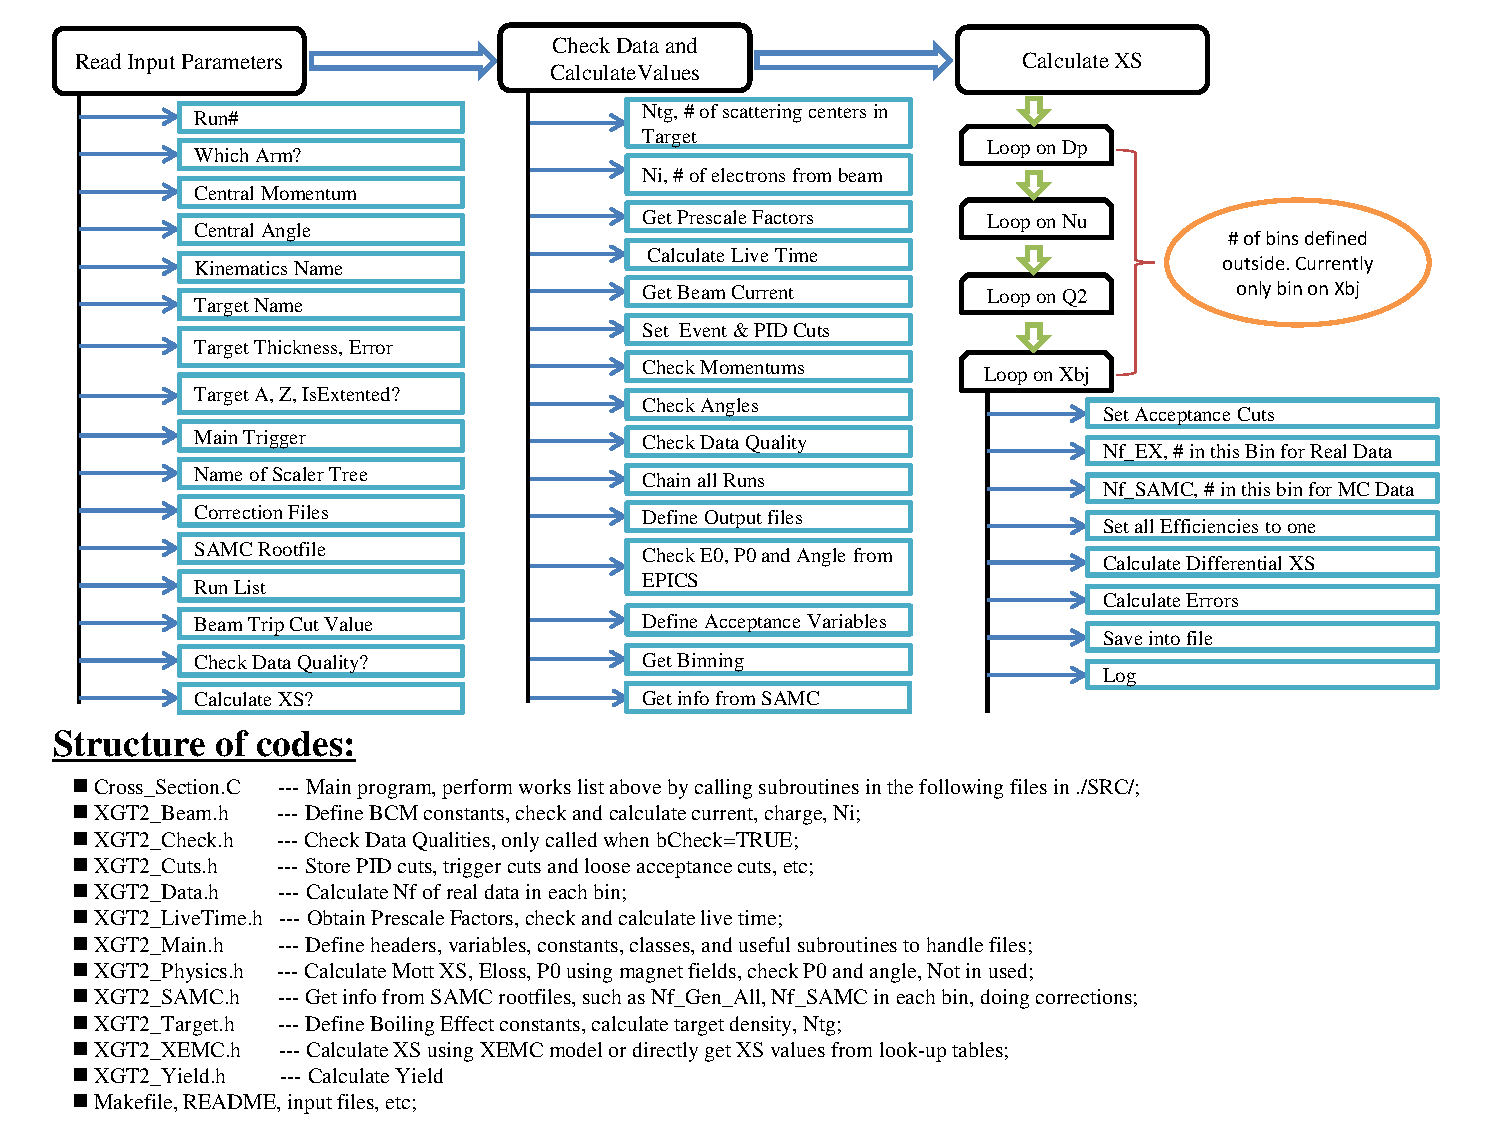
\includegraphics[type=pdf, ext=.pdf,read=.pdf,width=0.99\textwidth]{../figures/XS_Chart}
 \caption[Basic structure of XS package]{Basic structure of the cross section extraction package}
 \label{xs_chart}
\end{figure}

\subsection{Electron Beam Charge}
 With the BCM parameters calibrated by Patricia, we are able to calculate total electron charge delivered from the accelerator in each run. Normally we use the last reading of counts by a BCM scaler to calculate the charge recorded by this monitor. However, if we intend to eliminate events taken during beam trip, the amount of electron charge accumulated when the beam current was lower than requested values will need to be subtracted from the total charge. A script was written to calculate the values of charge and current between two consecutive scaler events, and to assign the values for all events taken during this time period. For example, the charge and current calculated base on beam charge monitor (BCM) $U_{1}$ for $ith$ scaler event are given by:
\begin{equation}
  \Delta C_{i}^{U_{1}} = C_{i+1}^{U_{1}} - C_{i}^{U_{1}},  I_{i}^{U_{1}} = \Delta C_{i}^{U_{1}}/(T_{i+1}-T_{i}),
\end{equation}
where $\Delta C_{i+1}^{U_{1}}$ gives the calibrated values of charge accumulated between two consecutive scaler events happening at CPU clock $T_{i+1}$ and $T_{i}$, of which the difference is normally set to three seconds. Values of charge and current for BCM $U_{1}, U_{3}, D_{1}$ and $D_{3}$ are calculated similarly. Then a beam trip cut will remove events taken during the current was low, and the total number of electrons from the beam for each run is re-evaluated:
\begin{equation}
  N_{e} = \sum_{i^{*}} \frac{1}{4}(\Delta C_{i^{*}}^{U_{1}}+\Delta C_{i^{*}}^{U_{3}}+\Delta C_{i^{*}}^{D_{1}}+\Delta C_{i^{*}}^{D_{3}})(\frac{1}{4}(I_{i^{*}}^{U_{1}}+I_{i^{*}}^{U_{3}}+I_{i^{*}}^{D_{1}}+I_{i^{*}}^{D_{3}})>I_{beam\_trip\_cut}),
  \label{eq_ne}
\end{equation}
where $i^{*}$ means summarizing scaler events with beam current $I_{i^{*}}$ higher than the cutting value $I_{beam\_trip\_cut}$, which we chose to be half of the value we requested during the experiment.

During the experiment, BCM scalers in HRS-L did not work properly so we only used the values of charge in HRS-R since scalers on both side shared the same signals from the beam.

\subsection{Targets}

\subsubsection{Boiling Effect}
Total number of scattering centers (or nuclei) in a target with its known thickness is given by:
\begin{equation}
 N_{tg} = \frac{\rho\cdot l \cdot N_{a}}{A},
 \label{eq_ntg}
\end{equation}
where $\rho$ is the target density in $g/cm^{3}$, $l$ is the effective target length in cm, $N_{a}$ is the Avogadro's number and A is the nuclear number of the target. For cryogenic long targets, $l$ should be equal to the effective length after cuts, instead of the design length.

Heat deposits in the target system when beam is on and cause the variation of target densities. This so called boiling effect are needed to be corrected:
\begin{equation}
  \rho_{cor} = \rho \cdot (1.0 - B \cdot I /100),
   \label{eq_tgrho}
\end{equation}
where $I$ and $B$ are the value of beam current and the boiling factor for a specific target, respectively. Study of boiling factors is performed by Patrica Solvignon %\ref{boiling_patricia}.

\subsubsection{Density Non-Linearity}
\begin{figure}[ht]
 \begin{center}
   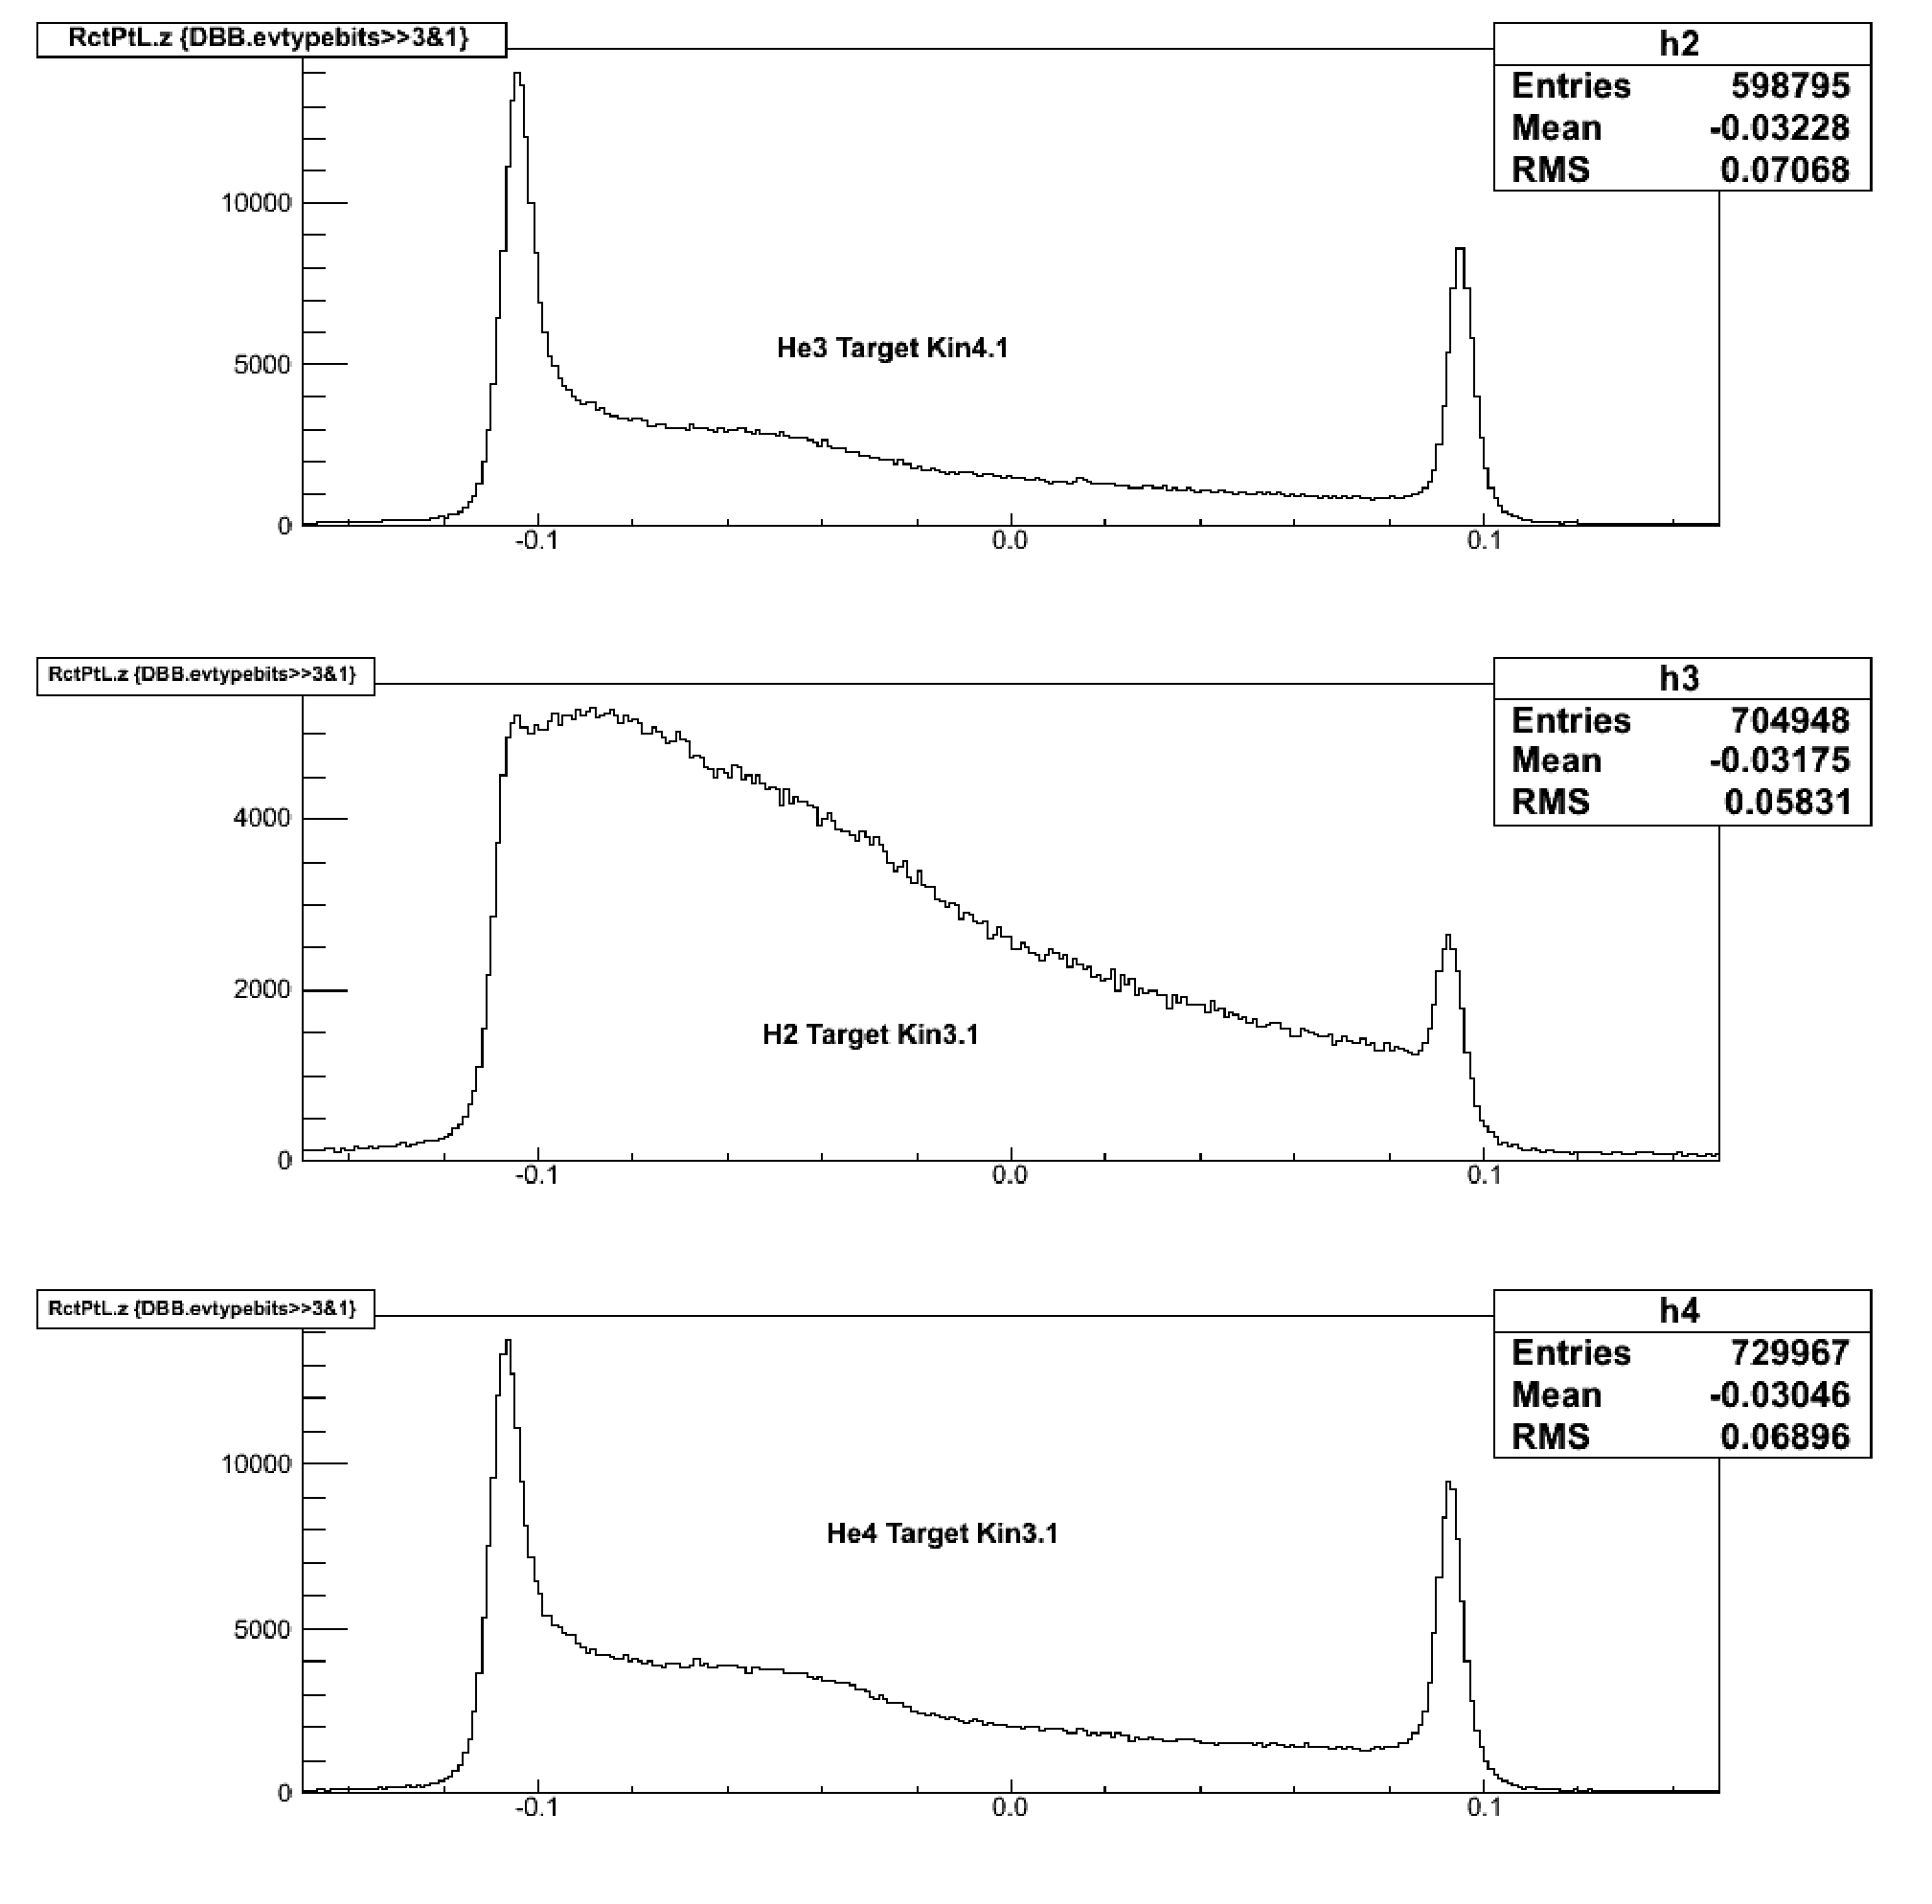
\includegraphics[type=pdf, ext=.pdf,read=.pdf,width=0.50\textwidth]{../figures/target/L_Cryo_RPZ}
  \caption[Long target bumps due]{Long target bumps due to non-uniform density distribution of $^{3}He$}
  \label{he3_bump}
 \end{center}
\end{figure}
During E08-014 experiment, we were using $20cm$ $^{2}H, ^{3}He$ and $^{4}He$ long cryogenic targets. The special design of cooling system caused targets having higher density upstream and lower density downstream, and the boundary of this two regions were at near $2cm$ toward upstream end-cup with a $4cm$ transition region. A bump clearly appears when plotting vertex distribution of one of those targets (Fig.\ref{he3_bump}), and the bumps become more significant when beam increasing (Fig.\ref{bump_current}).

\begin{figure}[!ht]
 \begin{center}
 \subfloat[$^{2}H$]{
   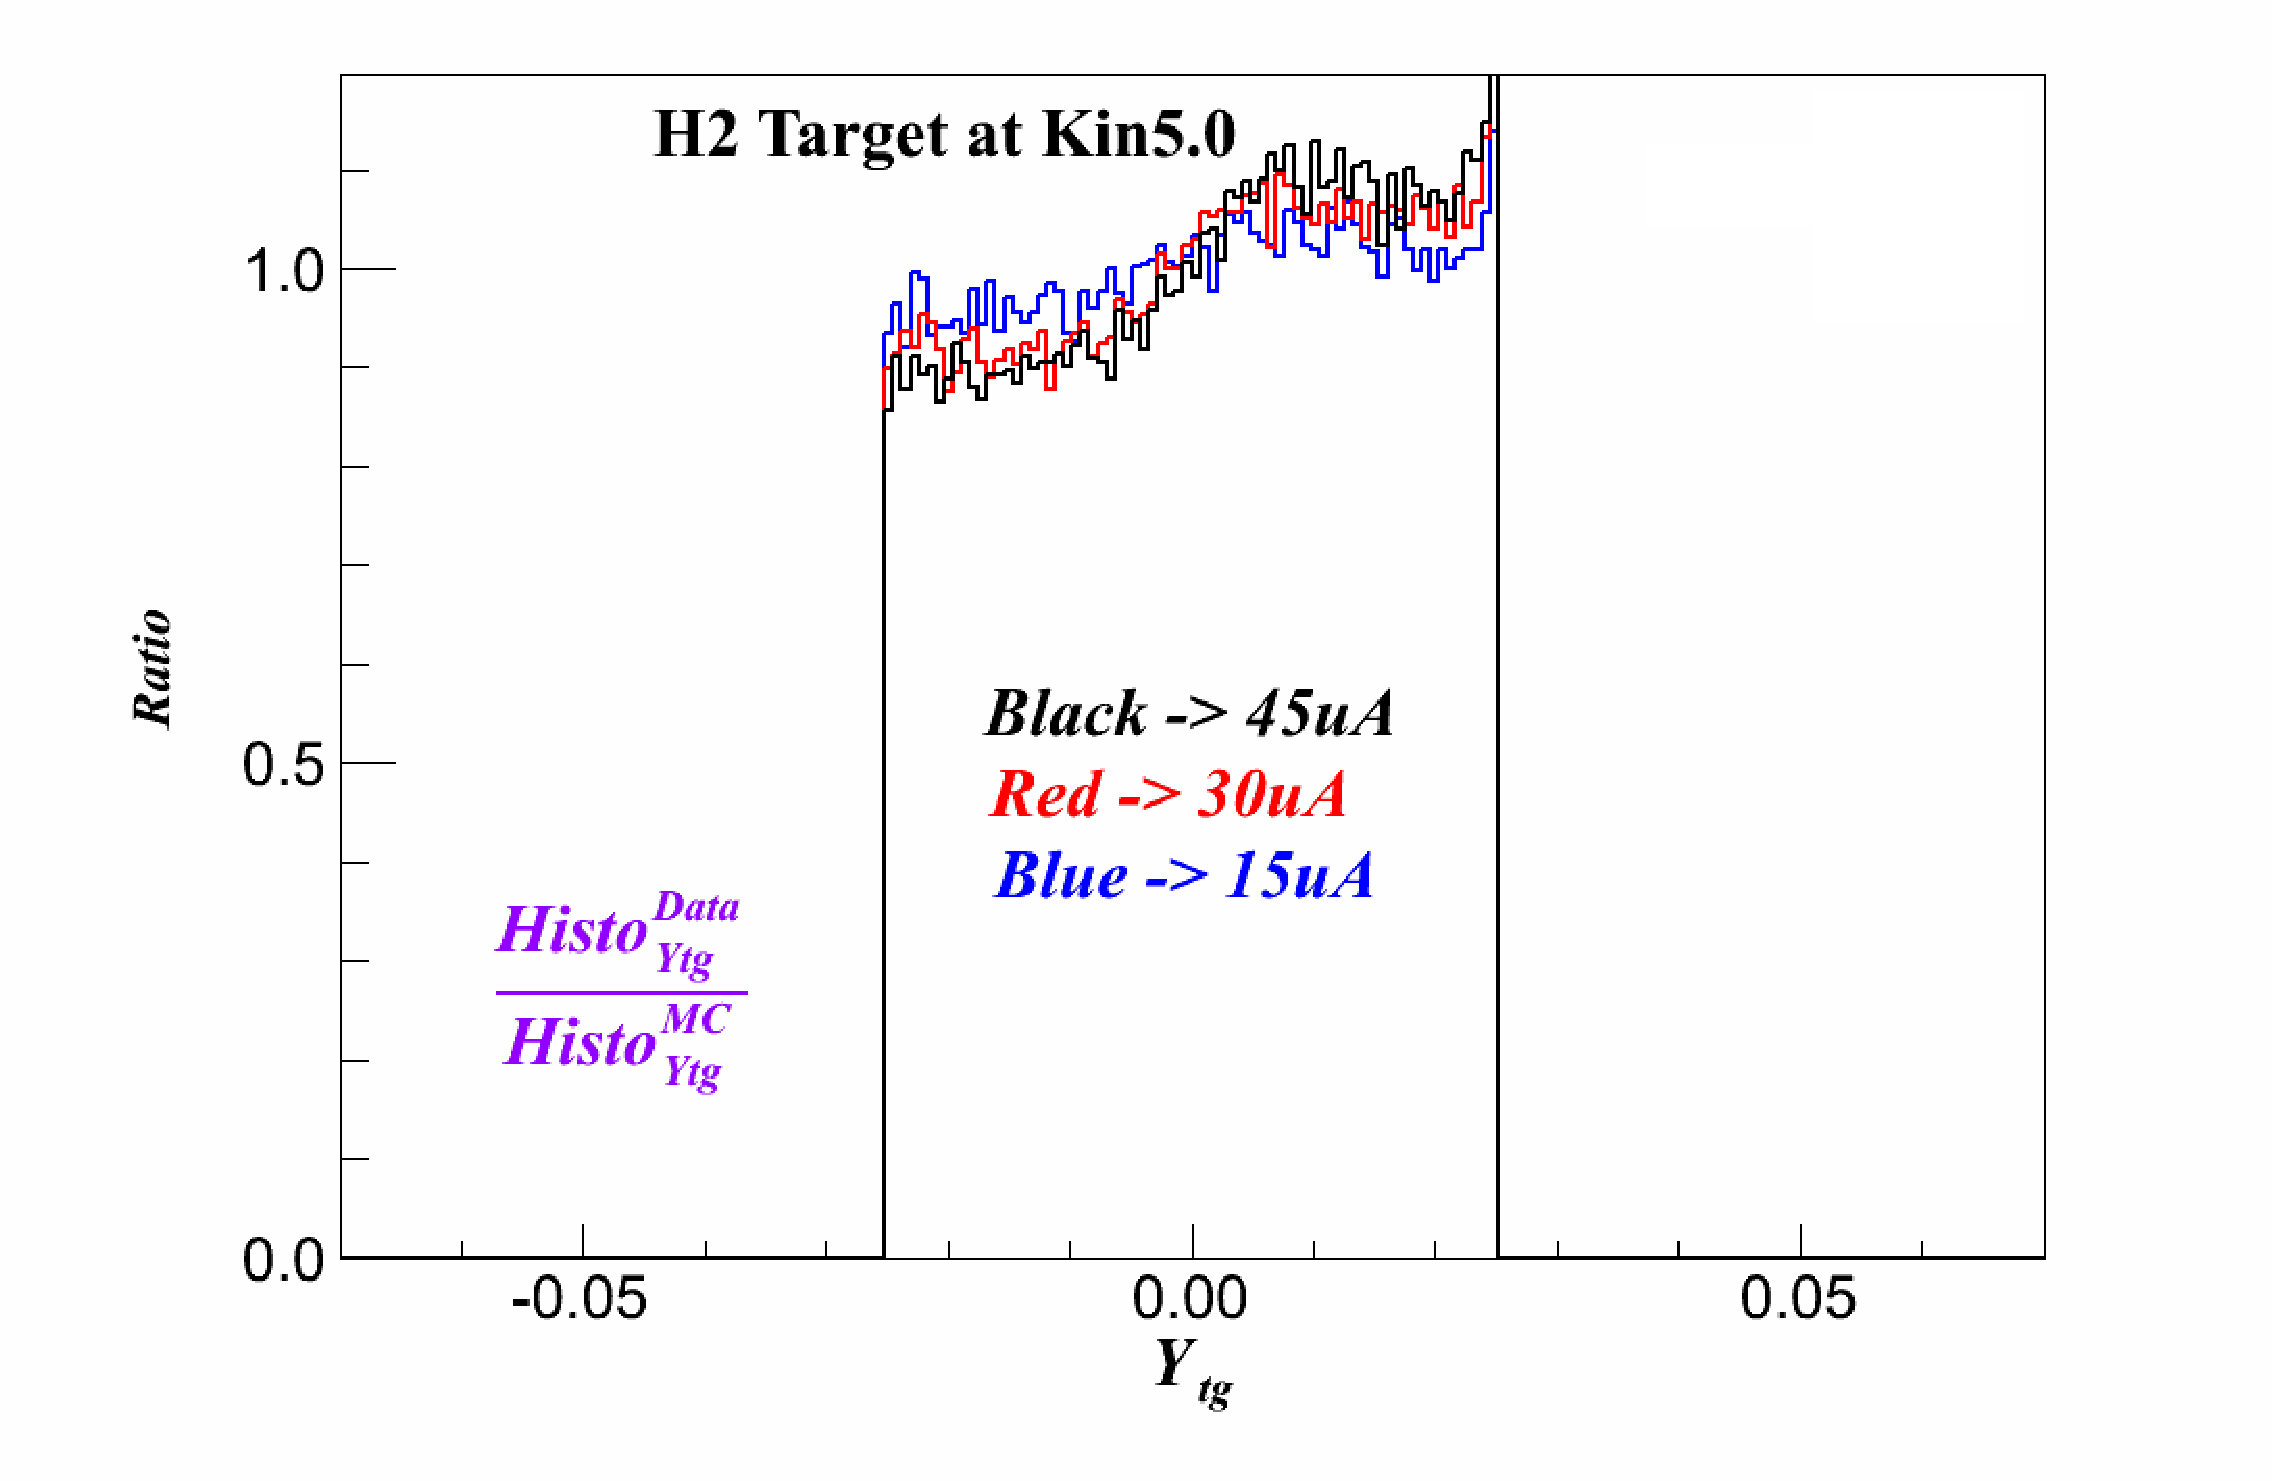
\includegraphics[type=pdf, ext=.pdf,read=.pdf,width=0.45\textwidth]{../figures/target/H2_Histo_Ratio}
 }
\hfill
 \subfloat[$^{3}He$]{
   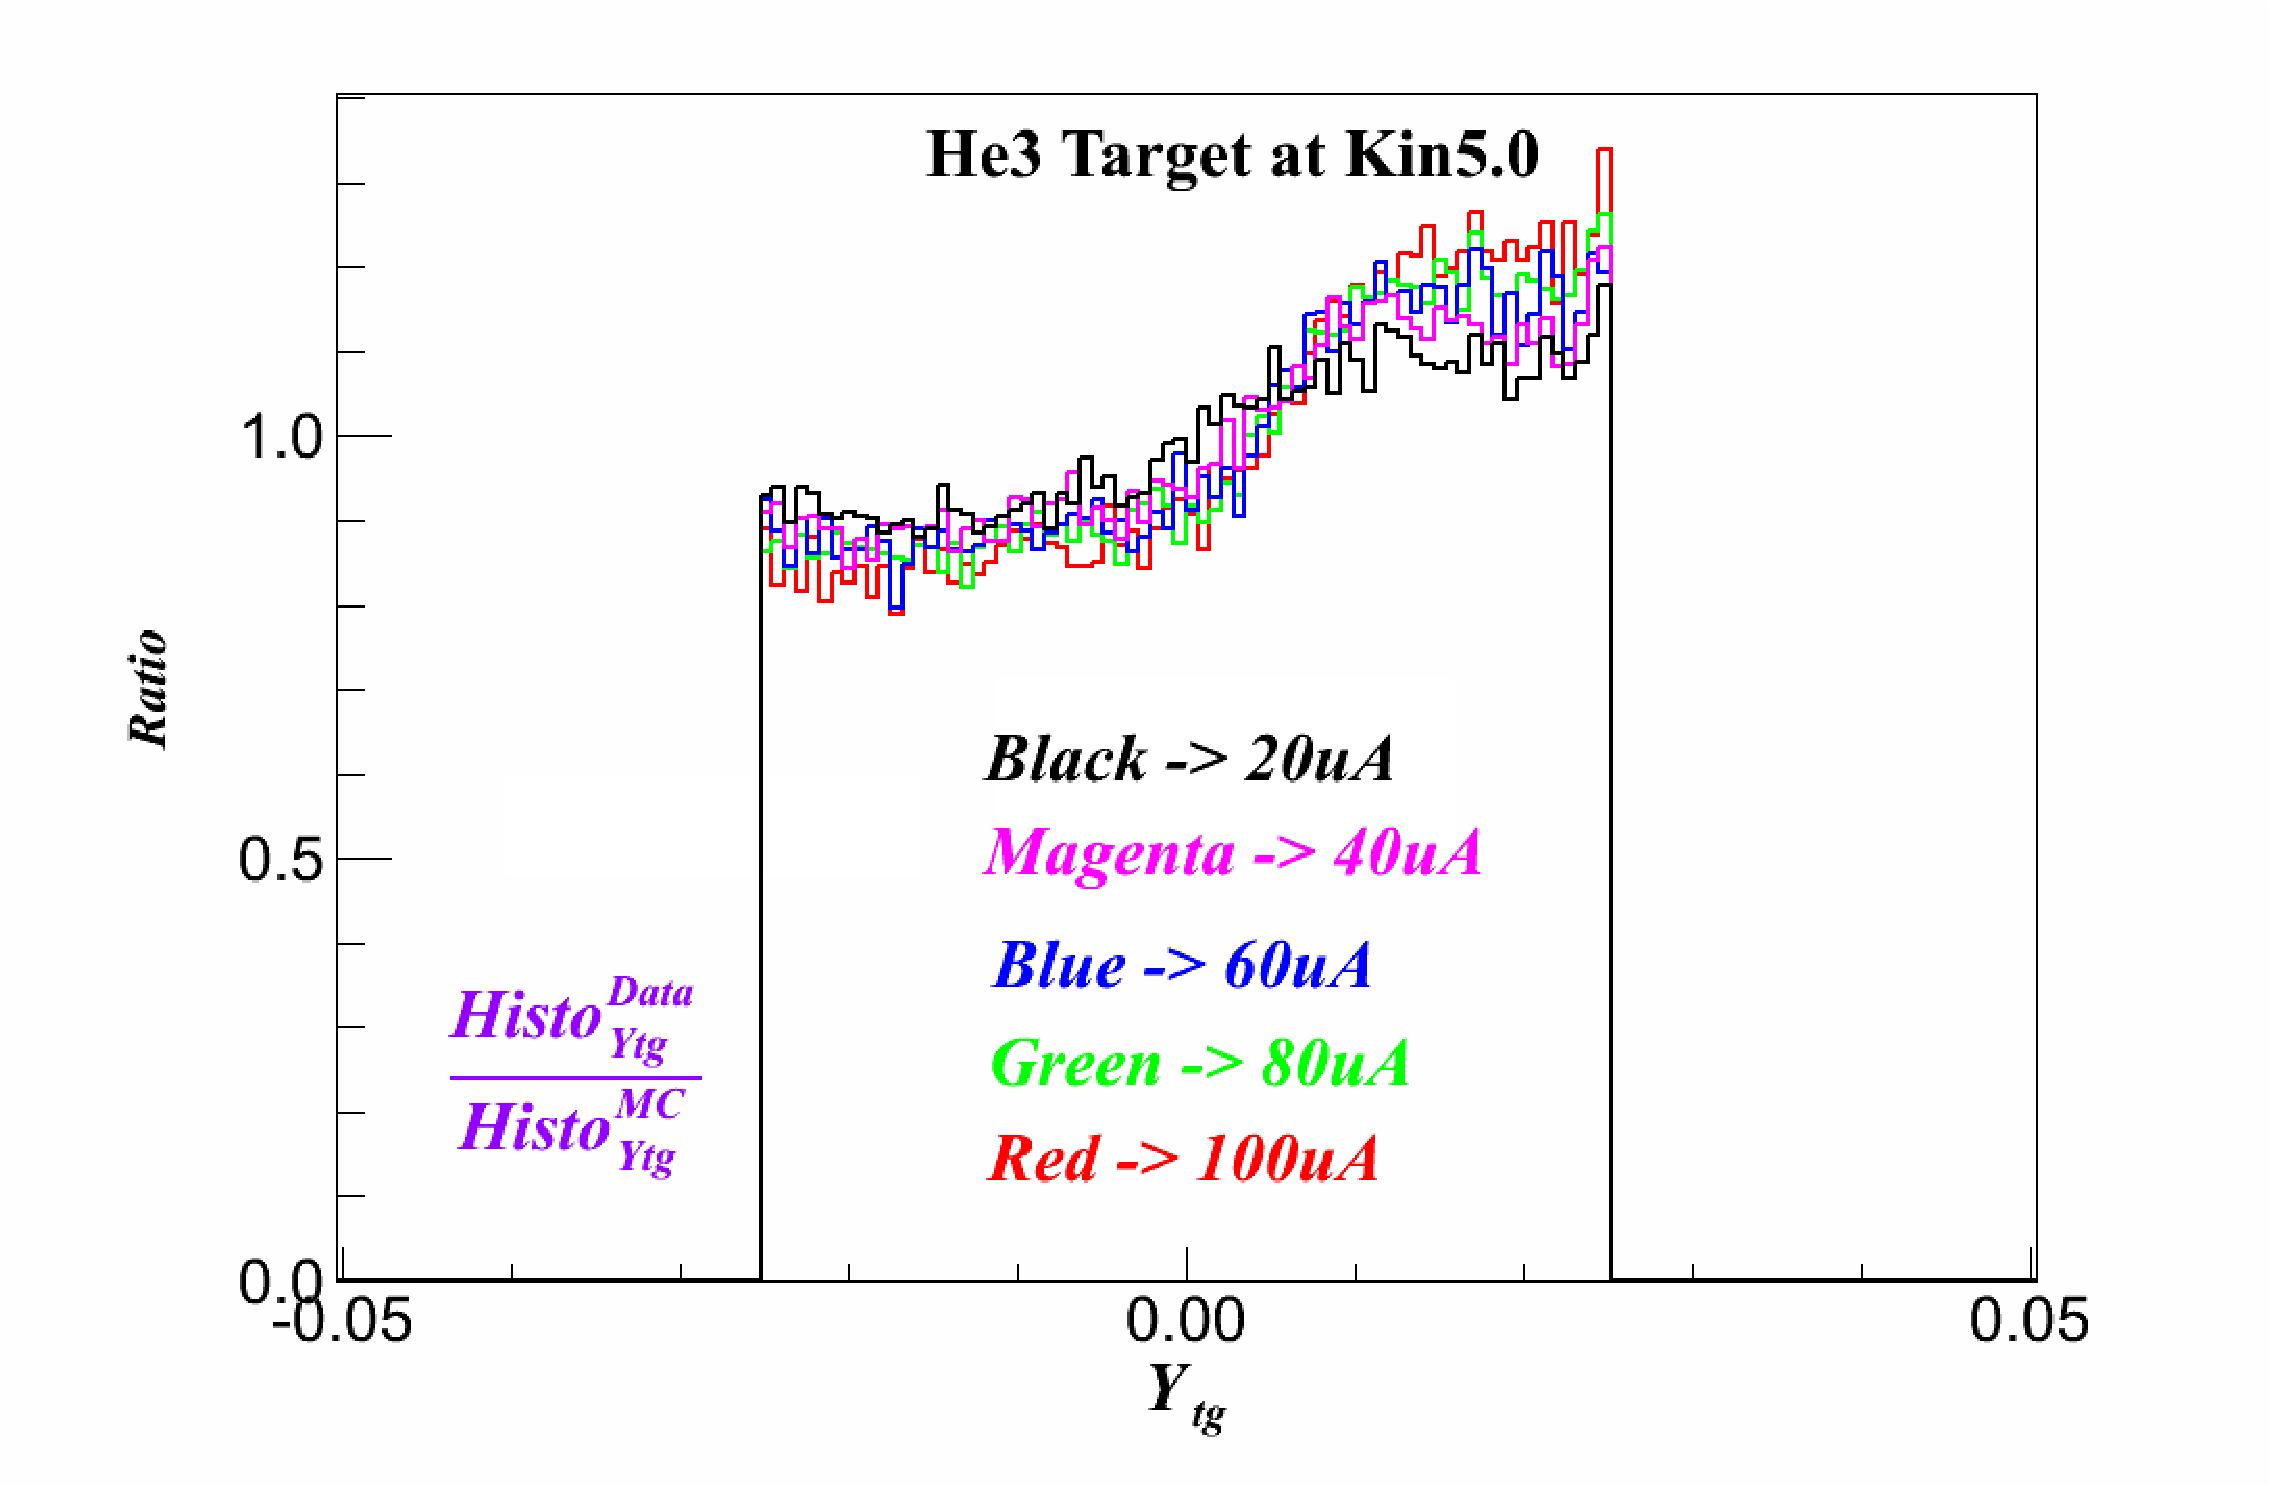
\includegraphics[type=pdf, ext=.pdf,read=.pdf,width=0.45\textwidth]{../figures/target/He3_Histo_Ratio}
}
\\
\subfloat[$^{4}He$]{
  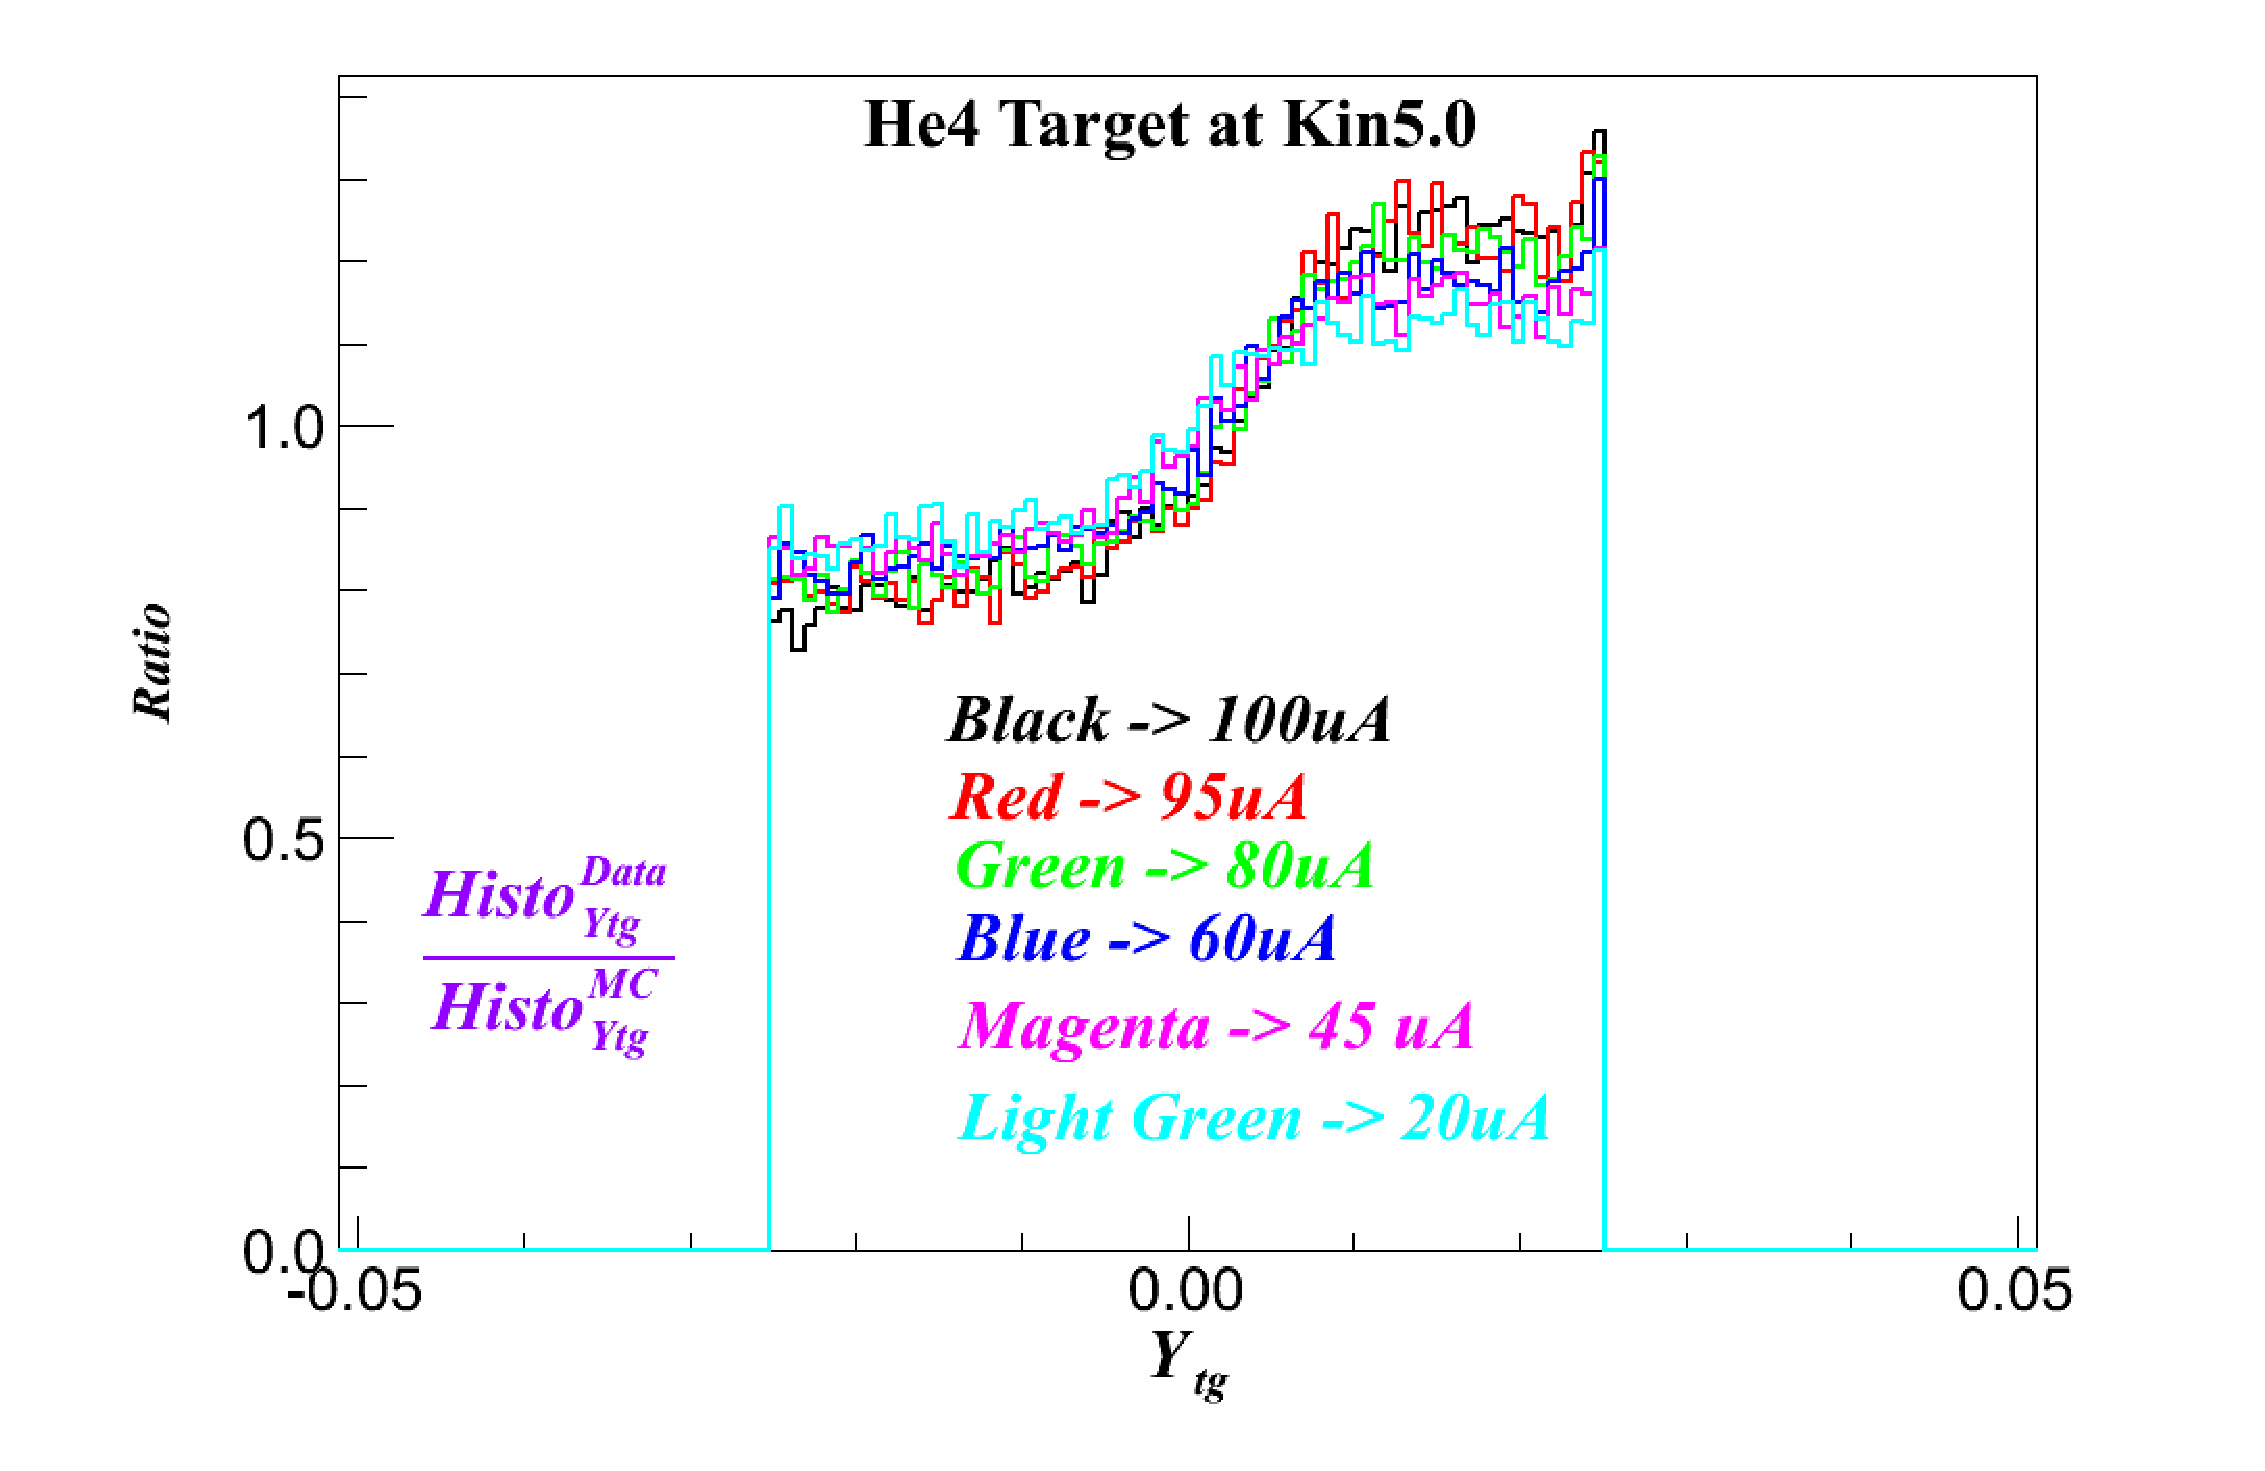
\includegraphics[type=pdf, ext=.pdf,read=.pdf,width=0.45\textwidth]{../figures/target/He4_Histo_Ratio}
}
 \caption[Long target bumps changing with beam current]{Long target bumps changing with beam current}
 \label{bump_current}
\end{center}
\end{figure}

The density non-uniformity of long targets causes several problems when extracting cross section results. First of all, instead of using average values of densities, total number of scattering centers is needed to be re-evaluated based on the distributions. Secondly, due to higher densities in the upstream part, a false physics phenomenal is introduced into the cross sections, and it has to be corrected since we don't bin on $Y_{tg}$. Last but not least, radiation correction will be much more complicate than one assuming the uniform target density since the the energy loss are more sensitive to the location of reaction points. A detail discussion will be given later about the methods to approach the problems using cross section models and Monte Carlo simulation.

\subsection{Live Time}

DAQ running at high trigger rates generally decreases live time, or increases dead time in other words. Dead time is mainly composed of hardware dead time and electronic dead time. Hardware dead time comes from the fact that detectors can not identify two or more particles coming nearly at the same time. Electronic dead time, which is the major source, arises when electronic modules, including computer system, skip the next event when they are still processing the current event, and cause those events not recorded by DAQ system. To reduce the dead time we assign a pre-scale factor to each trigger type to control the total trigger rates. The values of pre-scale factors are stored in each run and can be read out to calculate the actually total number of events from different triggers.

We can evaluate the electronic dead time by using the fact that events not recorded by DAQ are still counted by scalers. For each trigger type, the value of live time is given by the ratio of total number of events recorded by DAQ before prescaling and the total counts in scalers:
\begin{equation}
  LiveTime_{T_{i}} = \frac{N_{T_{i}}^{DAQ} PS_{T_{i}}}{N_{T_{i}}^{Scaler}},
  \label{eq_lt}
\end{equation}
where $N_{T_{i}}^{DAQ}$ and $N_{T_{i}}^{Scaler}$ are the total number of DAQ events and scaler counts in one run after the beam trip cut.

\subsection{Efficiencies}

Detectors do not work in 100\% performance and the inefficiencies of detectors caused by hardware and software are needed to be evaluated and corrected when extracting cross sections. The analysis results show that for E08014 data, the detection efficiencies of all detectors are very close to $99\%$ and meanwhile, loose PID cuts are good enough to eliminate most of pions and their cut efficiencies are also close to 99\%. So during the cross section calculation, we don't apply corrections of those efficiencies but only quote $1\%$ of the systematic errors.

% 
% \subsubsection{Triggers}
% \begin{figure}[!ht]
%  \begin{center}
%   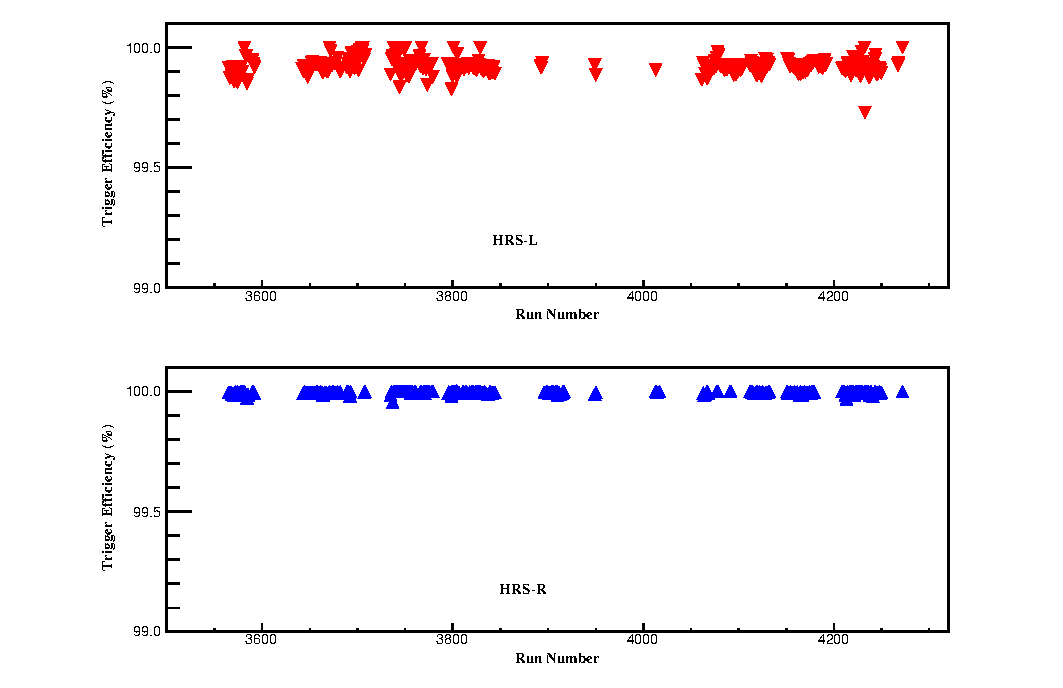
\includegraphics[type=pdf, ext=.pdf,read=.pdf,width=0.69\textwidth]{../figures/scin/Trigger_Eff}
% \captionof{figure}{\footnotesize{Trigger Efficiencies}}
%   \label{trig_eff}
%  \end{center}
% \end{figure}
%  There are mainly three aspects that determine the trigger efficiency~\cite{R_Bock}, first one of which is the trigger algorithm designed to compromise between highly reducing background and keeping most of good events, second one of which would be the dead time caused by electronics and performance of detectors involved in the trigger system, and the last one of which is the writing speed of computer systems. It is important to avoid double counting detectors' inefficiencies when evaluating trigger efficiencies. The definition of trigger efficiency generally includes the inefficiency of scintillator counters and the formula is written as:
% \begin{equation}
%  \epsilon_{trigger\_eff} = \frac{PS1(3)\times N_{T1(3)}}{PS1(3) \times N_{T1(3)}+PS2(4)\times N_{T2(4)}},
%  \label{trigger_eff}
% \end{equation}
% where $N_{T1(2,3,4)}$ is number of events triggered by T1(2,3,4) after prescaled by PS1(2,3,4). Traditionally in Hall-A T1(3) is designed by requesting coincidence trigger signals between S1 and S2m, while T2(4) includes signals from GC in the trigger, which should carry the inefficiency effect of GC. However, during the E08014 experiment, T1(3) was modified to include GC signals in trigger, so the detection inefficiency of GC is canceled from the equation. Fig.\ref{trig_eff} shows that the trigger efficiencies of our data on both arm were better than 99\%.
% 
% \subsubsection{VDCs}
% 
% Inefficiency of VDCs caused by hardware is negligible and the major source is from the mis-reconstruction of particle tracks during the tracking algorithm. Only one-track events are kept for analysis, and the good events threw away by zero-track and multi-tracks cut are corrected by the one-track efficiency defined as:
% \begin{equation}
%  \epsilon_{one\_track\_eff} = \frac{N_{Track=1}}{N_{0<=Tracks<=4}}
% \end{equation}
% It is very important to select correct electron samples when calculating values of one-track efficiency. We need to avoid applying cuts on variables that require tracking information, such as variables at focal plane and target plane, and cutting on other VDC variables will introduce other sources of inefficiencies. Cluster-reconstructed variables of calorimeters, such as E/P, can not be used when cutting electrons. cosmic ray events should also be removed since they come with big angles. We could not cut on TOF $\beta$ to suppress cosmic ray background due to the TDC multi-peaks issues on some scintillator bars. During the analysis, we used quasi-elastic carbon data which has low cosmic ray background due to the high rates,then applied cut on T1(3) trigger, GC ADC sum and Calorimeters ADC sum to select pure electron events, and we also require only one-hit on each scintillator bar for each event to remove events with multi-particles.From Table~\ref{vdc_table}, we obtained the fraction of one-track and multi-track events, which are above 99\% on each arm.
% \begin{table}[!ht]
% \centering
% \begin{tabular}{|c||ccccc|}
% 	\hline
% \textbf{Number of tracks}  & 0 & 1 & 2 & 3 & 4     \\
% 	\hline \hline
% HRS-L   & 0.0298\% & 99.1750\% & 0.7430\% & 0.0452\% & 0.0048\%  \\
%         \hline
% HRS-R   & 0.0482\% & 99.3600\% & 0.5446\% & 0.0388\% & 0.0073\%  \\
% 	\hline \hline
% \end{tabular}
% \caption{Fraction of different tracks events from quasi-elastic data,w/o $\beta$ cut}
% \label{vdc_table}	
% \end{table}
% 
% \subsubsection{PID detectors}
% \begin{figure}[!ht]
%  \begin{center}
%   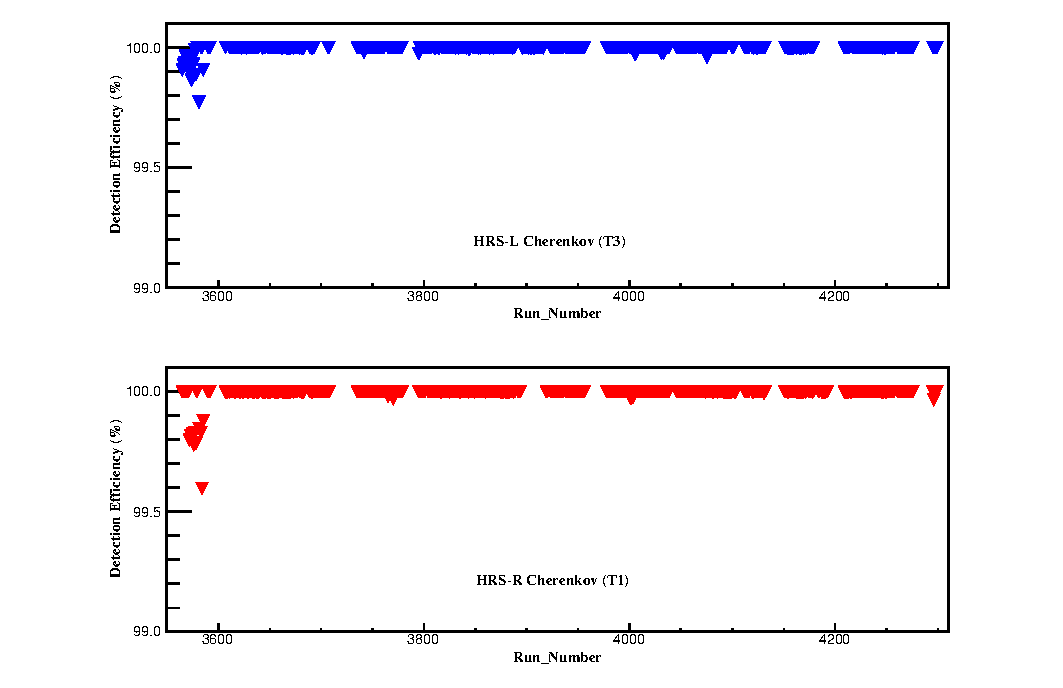
\includegraphics[type=pdf, ext=.pdf,read=.pdf,width=0.69\textwidth]{../figures/cer/Cer_Det_Eff}
%   \caption[Gas Cherenkov Detection Efficiency]{\footnotesize{Gas Cherenkov Detection Efficiency}}
%   \label{cer_det_eff}
%  \end{center}
% \end{figure}
% %\subsubsection{Gas Cherenkov}
% For Gas Cherenkov detectors and lead-glass Calorimeters, there are two parts of information needed to be extracted: the fractions of particles detected when they pass through the detectors and leave signals, or called detection efficiencies; and the percentages of electrons remaining and pions contaminating when applying PID cuts, also called PID-Cut efficiencies. PID-Cut efficiencies basically tangle with detection efficiencies due to the fact that we deal with detected events. We need to firstly evaluate detection efficiencies and PID-Cut efficiencies will be discussed in next section.
% 
% Detection efficiency of GC (Calorimeters) can be defined as:
% \begin{equation}
%  \epsilon_{detection\_eff}^{cer(calo)} = \frac{N_{detected}^{cer(calo)}}{N_{samples\_from\_calo(cer)}},
% \end{equation}
% where $N_{cer(calo)}$ is number of particles detected by GC (Calorimeters), and $N_{samples}$ is number of particle samples from Calorimeters (GC). During the analysis, we cut on T1(3) trigger and spectrometer acceptance, and pure electron were selected by applying cuts on main peaks of E/P spectra of Calorimeters when studying GC, or on the peaks of Cherenkov ADC Sum when studying Calorimeters.
% 
% The design of Hall A Gas Cherenkov detectors should give high detection efficiency, since electrons can easily trigger the detectors with very low threshold, while pions and other particles from cosmic ray can not fire the detectors directly, and the inefficiency is caused by particles hitting the edges of gas boxes or PMT tubes. Fig.\ref{cer_det_eff} shows that on both arm, the detection efficiencies of Gas Cherenkov detectors are close to 100\%.
% 
% %\subsubsection{Calorimeters}
%  The detection efficiencies of lead glass calorimeters are expected to be lower than Gas Cherenkov detectors. Calorimeters are composed by piles of lead glass blocks, so the inefficiency of detection is mainly from particles going through gaps in between blocks or hitting the edges or PMT tubes before cascade. Cluster reconstruction when calculating deposited energy in lead glass blocks is another source of inefficiencies, especially when the electron rate is low and many low energy cosmic ray particles mix in.From Fig.\ref{calo_det_eff}, we see that the detection efficiencies of calorimeters on both arm are still high than 99\% for most of runs, but for some runs with low electron rates, mainly for $^{3}He$ target with low beam current (Fig~\ref{calo_det_eff_mom}),the detection efficiencies are slightly lower, due to more cosmic ray contamination. Events from cosmic ray will eventually be removed by applying acceptance cuts and PID cuts, so no correction is necessary for those runs.
% \begin{figure}[!ht]
%  \begin{center}
%  \subfloat[vs Run Number]{
%   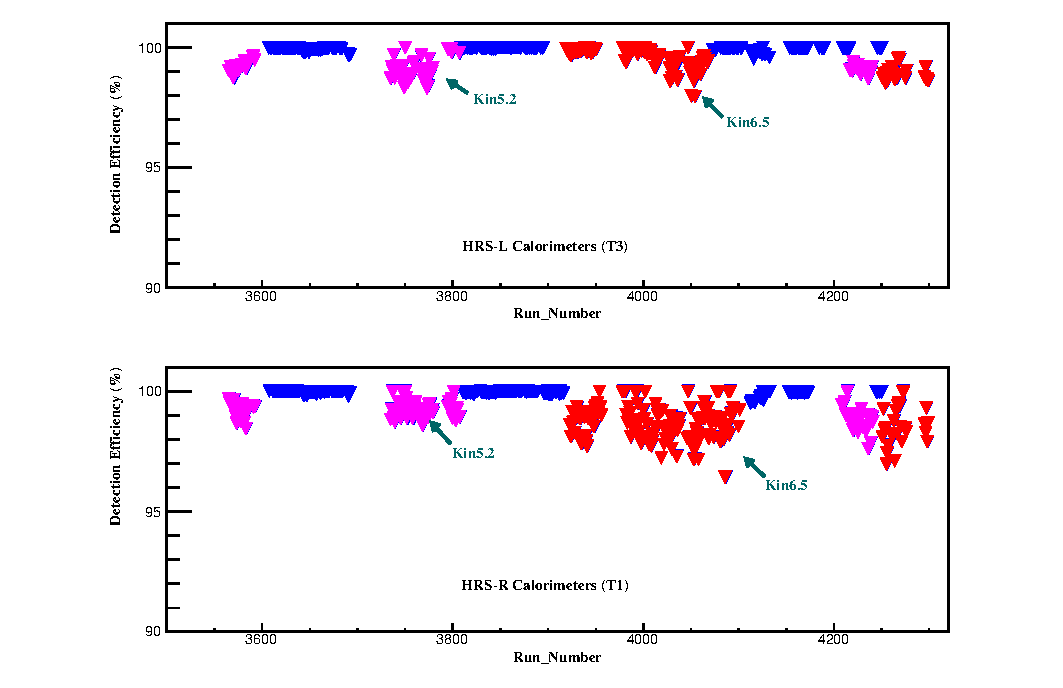
\includegraphics[type=pdf, ext=.pdf,read=.pdf,width=0.69\textwidth]{../figures/calo/Calo_Det_Eff1}
% }
% \\
%  \subfloat[vs Momentum]{
%   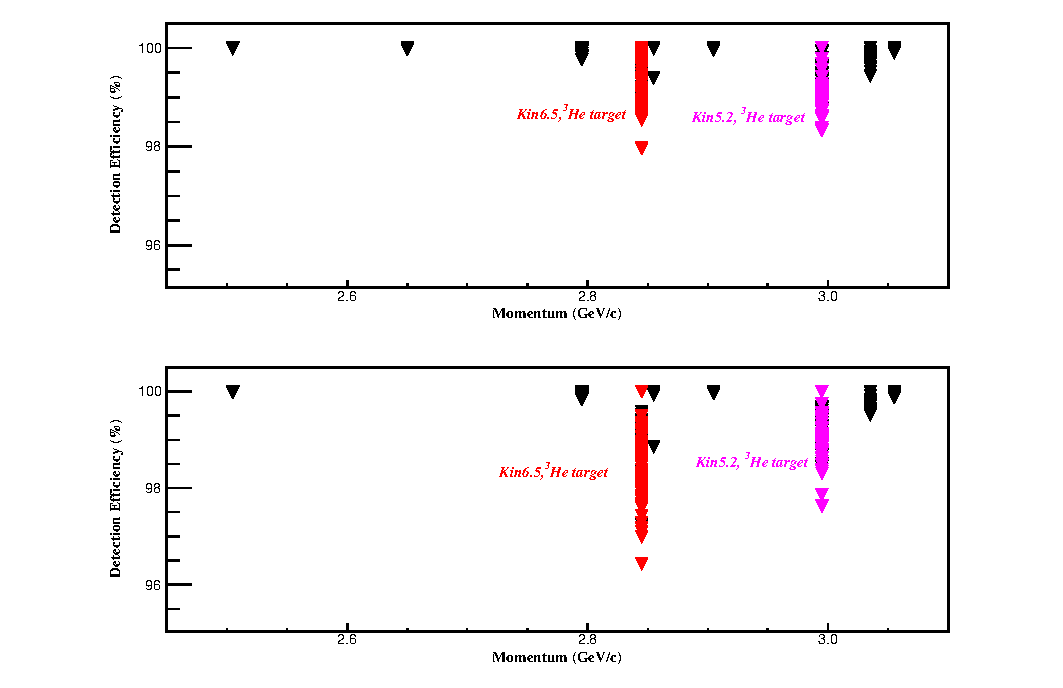
\includegraphics[type=pdf, ext=.pdf,read=.pdf,width=0.69\textwidth]{../figures/calo/Calo_Det_Eff_Mom1}
% }
%  \caption[Crlorimeters Detection Efficiencies]{\footnotesize{Calorimeters Detection Efficiencies. The first graphic shows the efficiencies are mostly above 99\%, while the second shows that runs with lower efficiencies are for gas targets at low production rates}}
%  \label{calo_det_eff}
%  \end{center}
% \end{figure}

\subsection{Acceptance and Binning}
 
\subsubsection{Acceptance}
We start with tight acceptance cuts on target plane variables, while the cuts on focal plane variables are reasonablly loose. We will generally open the cut on each target plane variables and study the variation of cross section values. Final values of acceptance cuts will fixed after the acceptance study (coming up).

\subsubsection{Binning}
 We currently bin on $x_{bj}$. The range and step size of binning is given in the following table:
\begin{table}[!ht]
\centering
\begin{tabular}{|c||ccccccc|}
  \hline
  \textbf{}        & Kin3.1 & Kin3.2 & Kin4.1 & Kin4.2 & Kin5.1 & Kin5.2 & Kin6.5 \\
  \hline \hline
  $x_{bj}^{Min}$   & 1.00   & 1.50   & 1.00   & 1.50   & 1.00   & 1.90   & 1.60   \\
        \hline
  $x_{bj}^{Max}$   & 2.30   & 3.00   & 2.30   & 3.00   & 2.30   & 3.00   & 3.00   \\
  \hline
  $x_{bj}^{Max}$   & 0.05   & 0.05   & 0.05   & 0.05   & 0.05   & 0.05   & 0.05   \\
  \hline \hline
\end{tabular}
\caption{Fraction of different tracks events from quasi-elastic data,w/o $\beta$ cut}
\label{bin_table}	
\end{table}

 Other binning methods, such as binning on $\delta p$, $\nu$ or $Q^{2}$ are also prepared in the code, and bin range and size are defined outside without modifying the code.

\subsection{Events Selections}

There are several cuts applied to select good scattered electron events, for example, for events in HRS-L:

\begin{enumerate}
\item \textbf{$DBB.evtypebits>>3\&1$}, cut on trigger events, $1$ for HRS-R and $3$ for HRS-L\\
\item \textbf{$DBB.edptl[0]==0$}, remove pulse events generated by EDTM modules
\item \textbf{$L.tr.n==1$}, only allow events with one track in VDCs \\
\item \textbf{$|x_{fp}|<=0.75 \&\& |y_{fp}|<=0.55 \&\& |\theta_{fp}|<=0.15 \&\& |\phi_{fp}|<=0.045$}, focal plane acceptance cuts \\
\item \textbf{$|\delta p_{tg}|<=0.03 \&\& |ReactPointZ|<=0.07 \&\& |\theta_{tg}|<=0.03 \&\& |\phi_{tg}|<=0.02$}, target plane acceptance cuts \\
\item \textbf{$L.cer.asum\_c>=50 \&\& epL<=0.5 \&\& L.prl2.e<=100$}, PID cuts for gas Cherekov detectors, and $E/P$ and second layer of calorimeters \\
\item \textbf{$left\_current >= I_{trip}$}, beam trip cuts \\
\item Binning Cuts
\end{enumerate}

The total number of events for a list of runs after the cuts defined above is given by:
\begin{equation}
  N_{EX}^{i} = \sum_{r} \frac{N_{T_{i}}^{r} PS_{T_{i}}^{r}}{LiveTime_{T_{i}}^{r}},
  \label{eq_nex}
\end{equation}
where $T_{i}$ defines the type of trigger we are interested in, $r$ represents one of runs in the list, $PS_{T_{i}}^{r}$ is the pre-scale factor of this trigger, and $N_{T_{i}}^{r}$ is the total number of events from $T_{i}$ and recorded by DAQ after cutting out beam trip.

\subsection{Cross Section Model}
The cross section model we used is called XEMC, which contains two parts: born cross section model and radiation corrections. There are two born cross section models, one of which is called QFS model\cite{temple_qfs}, and the other of which is adopted from XEM model\cite{xem} but we coded it in C++. We used the radiation correction subroutines developed by the group at Temple University. It is a very stand-alone package which can be called by other subroutines, and all parameters are defined outside, including materials of targets and windows, beam profile, spectrometer settings and so on. A option is given to do special treatment of density non-linearity of targets using in E08014.

\subsubsection{Born Cross Section Model}
 (QFS and XEM models comingup ...)
\subsubsection{Radiation Corrections}
 (RadC models coming up ...)

 It takes upto 7 minuites to calculate one radiated cross section value so a simplification is necessary if we need to generate many events. Considering that our kinematic settings are above the Quasi-Elastic region and the contribution from DIS part in the born cross section is small, we only use the QE part when calculating the radiation tail.

\subsubsection{Lookup Tables}
\begin{figure}[!ht]
 \begin{center}
  \includegraphics[type=pdf, ext=.pdf,read=.pdf,width=0.45\textwidth]{../figures/xemc/Table_LookUp}
  
  \caption[A sketch of cross section tables look-up]{\footnotesize{A sketch of cross section tables lookup. For a given setting ($E_{p}, \theta$), we fistly look for the lattice it belongs to, replace the angle value by the closest bin $\theta_{j}$, and use the linear algorithm to calculate the cross section values between $E_{p}^{j}$ and $E_{p}^{j+1}$.}}
  \label{xs_table}
 \end{center}
\end{figure}
For each target in each kinematics settings, we divided a large phase space ($\Delta\delta p=0.14$ and $\Delta\theta=0.20$) into $200 \times 200$ lattices and calculated the radiated cross section value in each lattice point. The bin size is fine enough for us to assume that in each $\delta p$ bin cross section values do not vary too much for difference $\theta$ values. Meanwhile, the distribution of cross section as function of $\delta p$ (or $E_{p}$) in each $\theta$ bin can be considered to be linear. Base on the assumptions, for an given event with ($E_{p}, \theta$), we look up the table (Fig~\ref{xs_table}), search for the most close angle value, $\theta^{i}$, as well as two momentum values,$E_{p}^{j}$ and $E_{p}^{j+1}$ (so $E_{p}^{j}<E_{p}<E_{p}^{j+1}$). We can obtain the estimated cross section value for this event using the linear relationship:
\begin{equation}
 \sigma(E_{p},\theta) = \sigma(E_{p}^{j},\theta^{i}) - \frac{E_{p}-E_{p}^{j}}{E_{p}^{j+1}-E_{p}^{j}}(\sigma(E_{p}^{j},\theta^{i})-\sigma(E_{p}^{j+1},\theta^{i}))
\end{equation}
We compared the difference between the table-lookup method and direct calculation, which is less than 0.1\%.


\subsection{Monte Carlo Simulation}
We used Hall-A Single Arm Monte Carlo (SAMC) to study the acceptance effect of HRSs and perform cross section corrections. SAMC was originally developed by A. Deur \cite{A_Duer} using FORTRAN and then converted into C++ by Huan Yao \cite{Huan_Yao}. For each simulation event, its quantities on the target plane, $x_{tg},y_{tg}, \theta_{tg}, \phi_{tg}$ and $\delta p_{tg}$, are uniformly generated in a wide phase space. A forward transportation function defines the geometry of each HRS and transports the target plane variables to the focal plane if this event can pass through. The calculated focal plane variables are further smeared by introducing VDCs' resolutions, then reconstructed back to the target plane using a back-forward transportation function. Meanwhile, physics quantities, including cross sections, can also be calculated by directly calling XEMC if the option is given. For our analysis, we turned off the physics module and obtained radiated cross sections values from the look-up tables instead.

Fig~\ref{samc_tg} compare the distribution of target plane variables between simulation data and experiment data for $^{12}C$ and $^{3}He$, where for simulation data all distributions are weighted by cross sections. Note that for $^{3}He$ target, the well known bump on the vertex distribution can be seen clearly when comparing with simulation data.

\begin{figure}[!ht]
 \begin{center}
 \subfloat[$^{12}C$]{
  \includegraphics[type=pdf, ext=.pdf,read=.pdf,width=0.44\textwidth]{../figures/samc/C12_Com_TG}
 }
\hfill
 \subfloat[$^{3}He$]{
  \includegraphics[type=pdf, ext=.pdf,read=.pdf,width=0.44\textwidth]{../figures/samc/He3_Com_TG}
}
 \caption[Comparing MC data and experiment data]{Comparing target plane variables of MC data (blue) and experiment data (red)}
 \label{samc_tg}
\end{center}
\end{figure}
  
In Eq.\ref{eqymc}, when calculating $\sum_{j\in i}\sigma^{rad}_{model}(E'_{j},\theta_{j})$ in the $ith$ $x_{bj}$ bin, we used the exact cut conditions as one in experimental data. A special correction for long targets in the simulation data will be discussed later.

\subsection{Calculation of Errors}
 In the cross section extraction package, a new type of variable is defined by a C++ class $XGT2\_VAR$, which not only includes the exact value of one quantity but also includes its sysmatic error and statistic error. When a new quantity is calculated from the operation of other quantities, all sysmatic errors and statistic errors from them will be seperately combined and carried by this new quantity. Comparing with evaluation of total errors after we exact the cross section values, this step-by-step method has its advantage to avoid mistakes such as miss-counting or multi-counting. The detail explaination of errors calculation and propagation is given as follows.

\subsubsection{Statistic Errors}
The detail of Statistic Errors are calculated as following:
\begin{enumerate}

\item \textbf{$N_{e}$:} From Eq.\ref{eq_ne}, since the charge is obtained from the average of four BCM monitor outputs ($u_{1},u_{3},d_{1}$ and $d_{3}$),the error is also averaged:
\begin{eqnarray*}
  \delta N_{e}^{r} &=& \sqrt{\frac{(\delta N_{e}^{r,d_{1}})^{2}+(\delta N_{e}^{r,d_{3}})^{2}+(\delta N_{e}^{r,u_{1}})^{2}+(\delta N_{e}^{r,u_{3}})^{2}}{4}}\\
                  &=& \sqrt{\frac{N_{e}^{r,d_{1}}+N_{e}^{r,d_{3}}+N_{e}^{r,u_{1}}+N_{e}^{r,u_{3}}}{4}}\\
                  &=& \frac{\sqrt{N_{e}^{r}}}{2} \\
\end{eqnarray*}
Hence,
\begin{equation}
  \delta N_{e} = \sqrt{\sum_{r}(\delta N_{e}^{r})^{2}}=\frac{1}{2}\sqrt{\sum_{r}N_{e}^{r}}=\frac{1}{2}\sqrt{N_{e}},
\end{equation}
where, $r$ means the run number.

\item \textbf{$Leve Time:$} Form Eq.\ref{eq_lt},
\begin{equation}
  \delta LT^{r}_{T_{i}} = LT^{r}_{T_{i}} \cdot \sqrt{\frac{1}{N_{T_{i}}^{DAQ} PS_{T_{i}}}+\frac{1}{N_{T_{i}}^{Scaler}}},
\end{equation}
where there is one thing that confuses me, which is that whether I should multiply $PS_{T_{i}}$ in the first term or not. It won't give us problem so far since most of runs have PS equal to one.

\item \textbf{$N_{EX}:$} From  Eq.\ref{eq_nex} and $N_{EX}=\sum_{r}N_{EX}^{r}$ for all runs, we have:
\begin{equation}
  \delta N_{EX}^{r} = N_{EX}^{r} \cdot \sqrt{\frac{1}{N_{T_{i}}^{r} PS_{T_{i}}} + (\frac{\delta LT_{T_{i}}^{r}}{LT_{T_{i}}^{r}})^{2} }, \delta N_{EX}=\sqrt{\sum_{r}(\delta N_{EX}^{r})^{2}}
\end{equation}

\item \textbf{$Y_{EX}:$} From Eq.\ref{eqyex},
\begin{equation}
  \delta Y_{EX} =  Y_{EX} \cdot \sqrt{(\frac{\delta N_{EX}}{N_{EX}})^{2}+(\frac{\delta N_{e}}{N_{e}})^{2}+(\frac{\delta\epsilon_{eff}}{\epsilon_{eff}})^{2}},
\end{equation}
where $\epsilon_{eff}$ is set to one and its statistic error and sysmatic error are set to zero and 1\%, respectively.

\item \textbf{$Y_{MC}:$} From Eq.\ref{eqymc},
\begin{equation}
  \delta Y_{MC} =  Y_{MC} \cdot \sqrt{(\frac{\delta\sum_{j\in i}}{\sum_{j\in i}})^{2}+(\frac{\delta N_{MC}^{gen}}{N_{MC}^{gen}})^{2}},
\end{equation}
where $\delta\sum_{j\in i} = \sum_{j\in i}\cdot\frac{1}{\sqrt{N_{MC}^{i}}}$, since it is sumarizing the cross section values of MC events ($N_{MC}^{i}$) in one bin.

\item \textbf{$\sigma_{EX}^{born}:$} From Eq.\ref{eqxs},
  \begin{equation}
  \delta \sigma_{EX}^{born} = \sigma_{EX}^{born} \cdot \sqrt{(\frac{Y_{EX}}{Y_{EX}})^{2}+(\frac{Y_{MC}}{Y_{MC}})^{2}}
\end{equation}

\end{enumerate}

\subsubsection{Systematic Errors}

\begin{enumerate}

\item \textbf{$N_{tg}$:}  Form $N_{tg} = \frac{\rho\cdot l \cdot N_{a}}{A}$, and $\rho_{cor} = \rho \cdot (1.0 - B \cdot I /100)$, there are three terms that can introduce errors: beam current measurement and calculation ($\delta I$), acuracy of Boiling Factors ($\delta B$), and the acuracy of target thickness measurement ($\delta \rho$). Last term is known but I temperately set the first two terms to zero. Hence:
 \begin{equation}
    \delta N_{tg} = \frac{\delta\rho}{\rho} \cdot N_{tg}
 \end{equation} 
\item \textbf{$N_{tg}$:}  1\% sysmatic errors is assigned to VDC One-Track efficiency, trigger efficiency, detection and cut efficiencies of Gas Cherenkov and Calorimeters, which add up to be 
\end{enumerate}

%\subsection{Cross Section Results}

\subsection{How to understand and work with the bumps}

Before we are able to directly calculate the absolute density distributions and hence evaluate the correct total number of scattering centers, we can estimate this distribution from real data with the help of cross section models and simulation data. The vertex distribution along beam direction ($ReactionPoint.Z$) not only includes the information of density distribution, but also contains the acceptance effect and cross section weighting. Since the simulation data with a good cross section model can reproduce close distributions of target variables (Fig.\ref{samc_tg}), and in the simulation we choose uniform target densities, a ratio of normalized histograms filled by real data and simulation data should be able to remove the acceptance effect and physics and the distribution of the ratio histogram should relatively represent the density distribution of the target (Fig.\ref{long_target_dis}).

\begin{figure}[ht]
 \begin{center}
  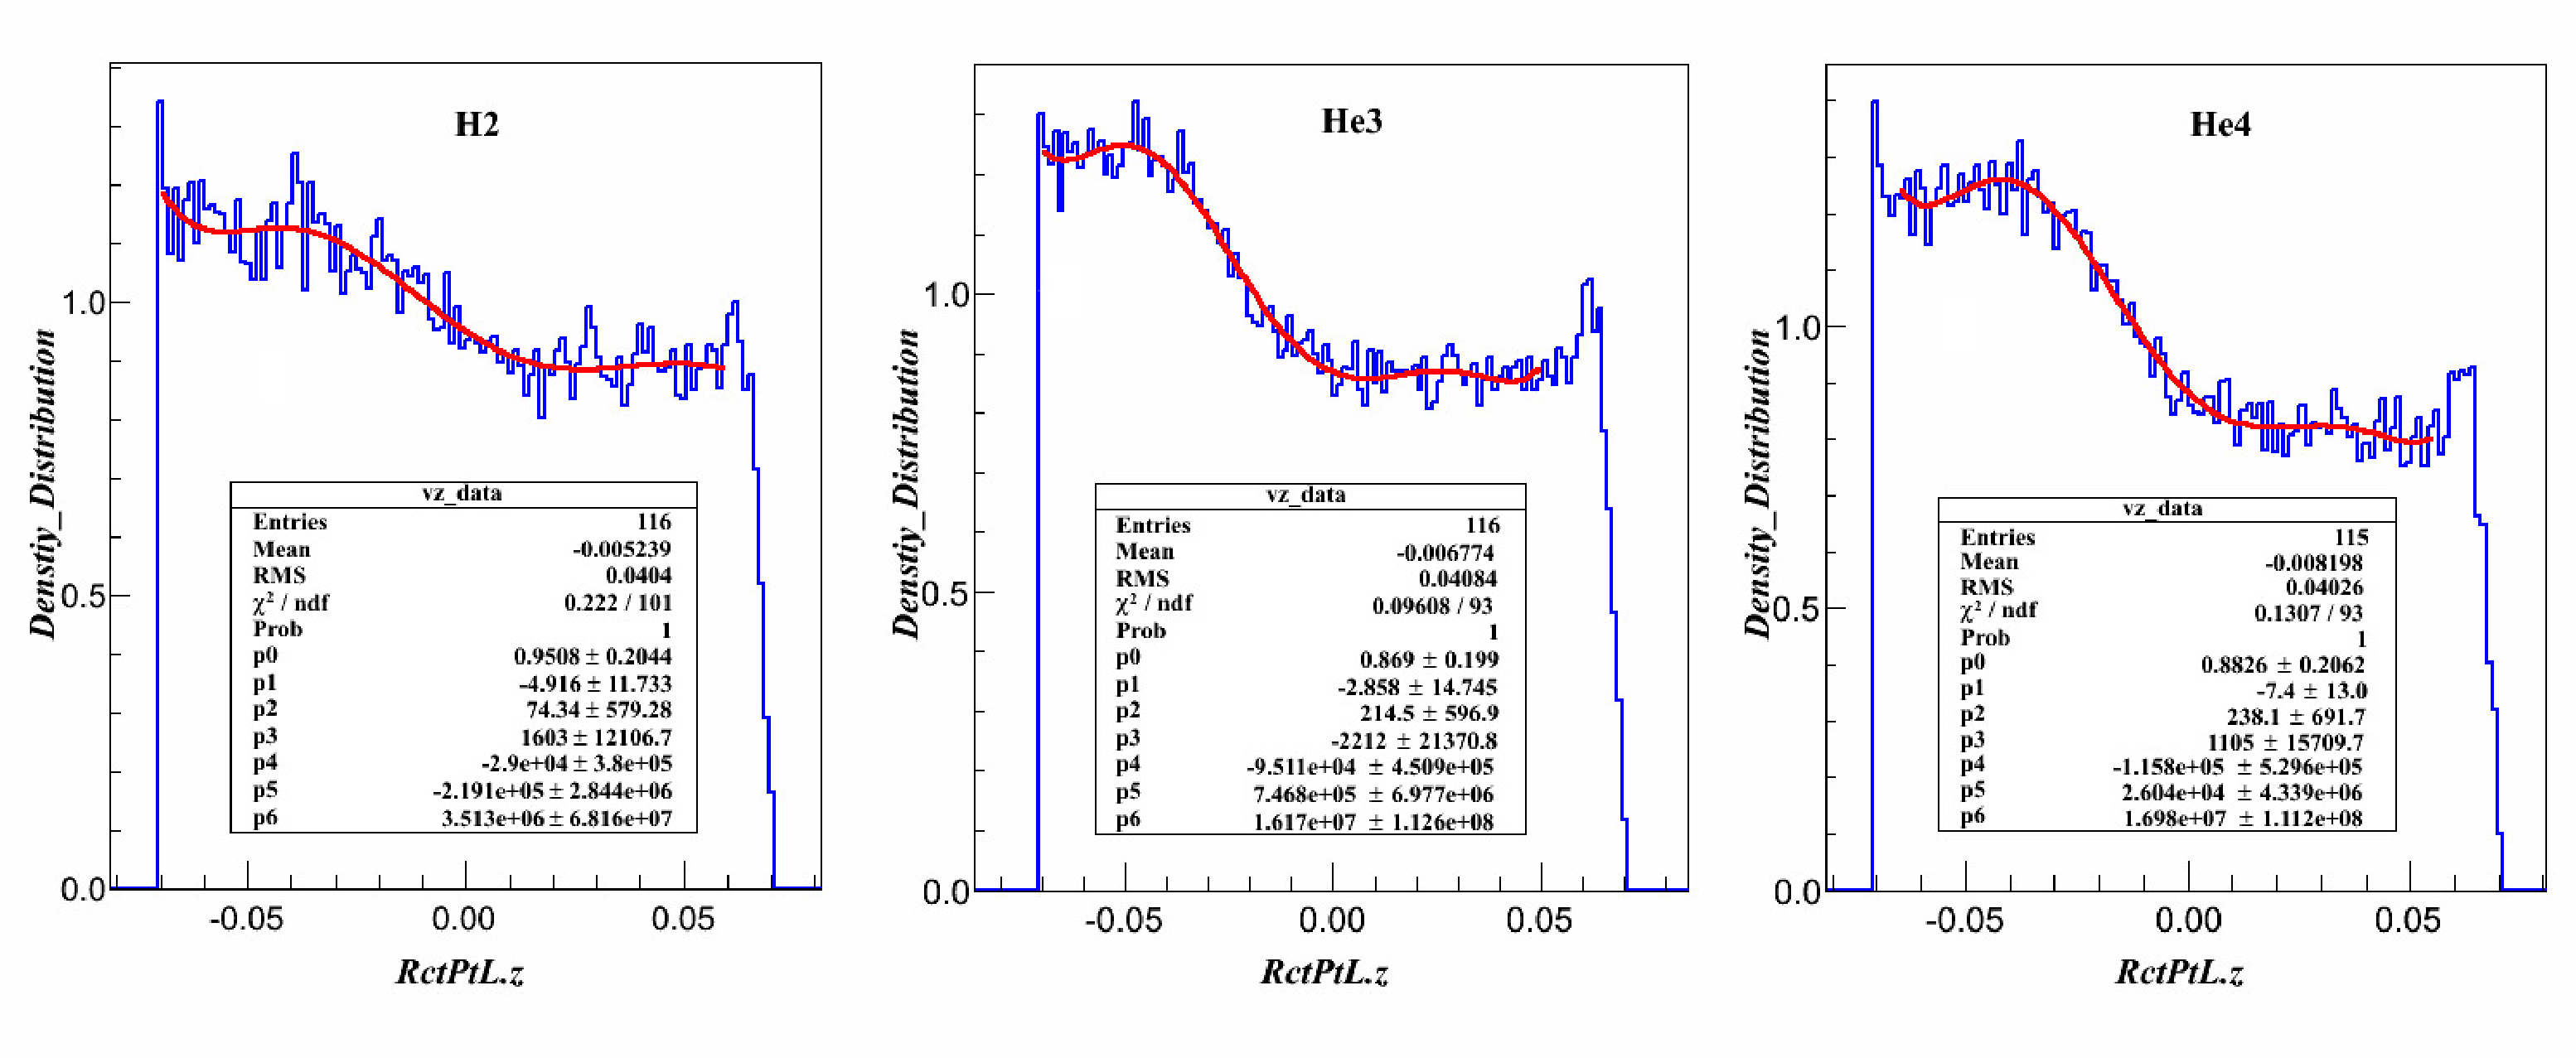
\includegraphics[type=pdf, ext=.pdf,read=.pdf,width=0.44\textwidth]{../figures/target/Target_Bump_Fit}
  \caption[Density distribution of long targets extracted from data]{Density distribution of long targets extracted from data}
  \label{long_target_dis}
 \end{center}
\end{figure}

 From the plots, we concludes that the density of upstream part is roughly 1.25 times larger than the average value while the downstream parts is roughly 0.85 times lower, and the boundary is not that clear. I wrote a step function and introduced the resolution of Vertex Z base on the quantity of optics reconstruction, and compared it with real data, and as you can see from Fig.\ref{long_target_step}, the transaction area does not agree well, which indicates that the target system is more complicate that what we thought.

\begin{figure}[ht]
 \begin{center}
  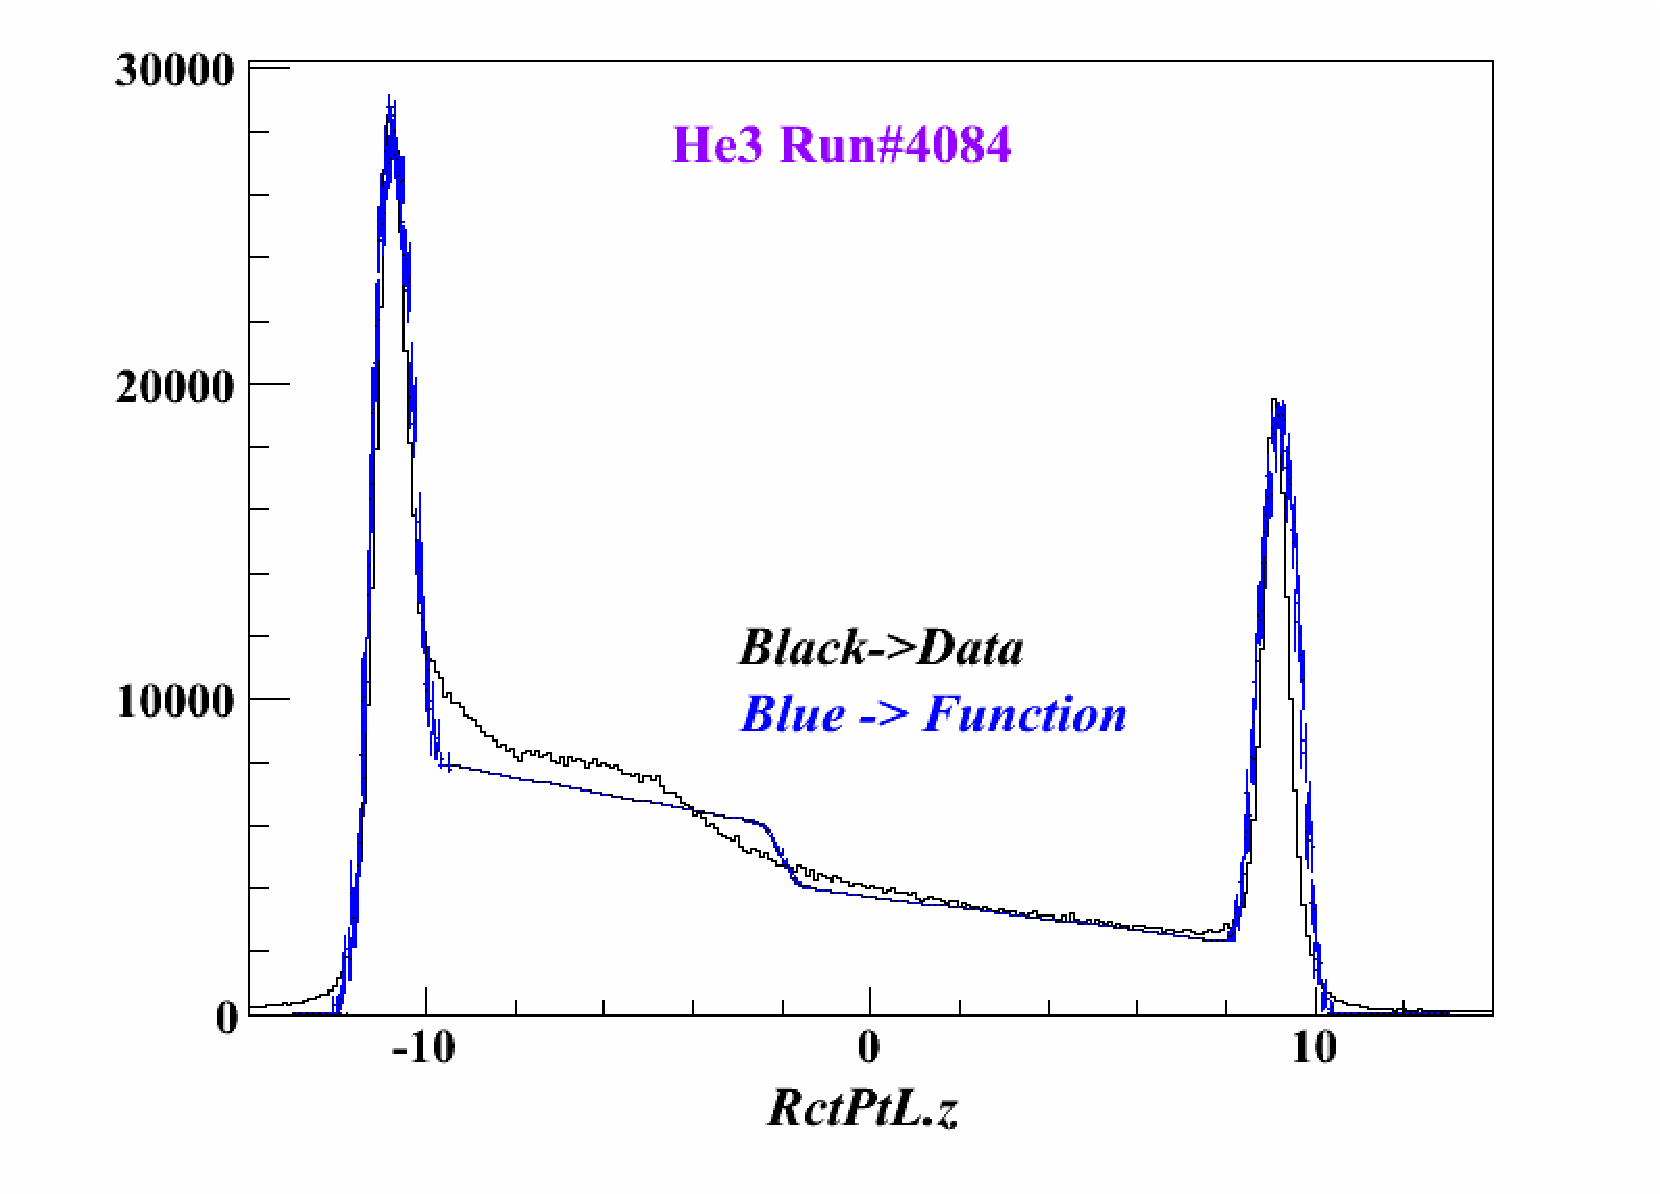
\includegraphics[type=pdf, ext=.pdf,read=.pdf,width=0.44\textwidth]{../figures/target/VZ_Com_True_Resol}
  \caption[Test the density distribution with a step function]{Test the density distribution with a step function}
  \label{long_target_step}
 \end{center}
\end{figure}

The other aspect we need to consider is that whether the non-linearity of long targets affects the distribution of cross section when binning on $x_{bj}$, which depends on scattering angles and hence indirectly depends on target vertex (or equally $Y_{tg}$). We look at the simulation data ($^{3}He$ at Kin3.1) and find out that -- if we make reasonable acceptance cuts and in a fine bin ($\Delta x_{bj} = 0.1$), the distribution of $Y_{tg}$ is flat which indicates that the Yield in one bin does not affected by the bump.

\begin{figure}[!ht]
 \begin{center}
 \subfloat[w/o acceptance cuts]{
  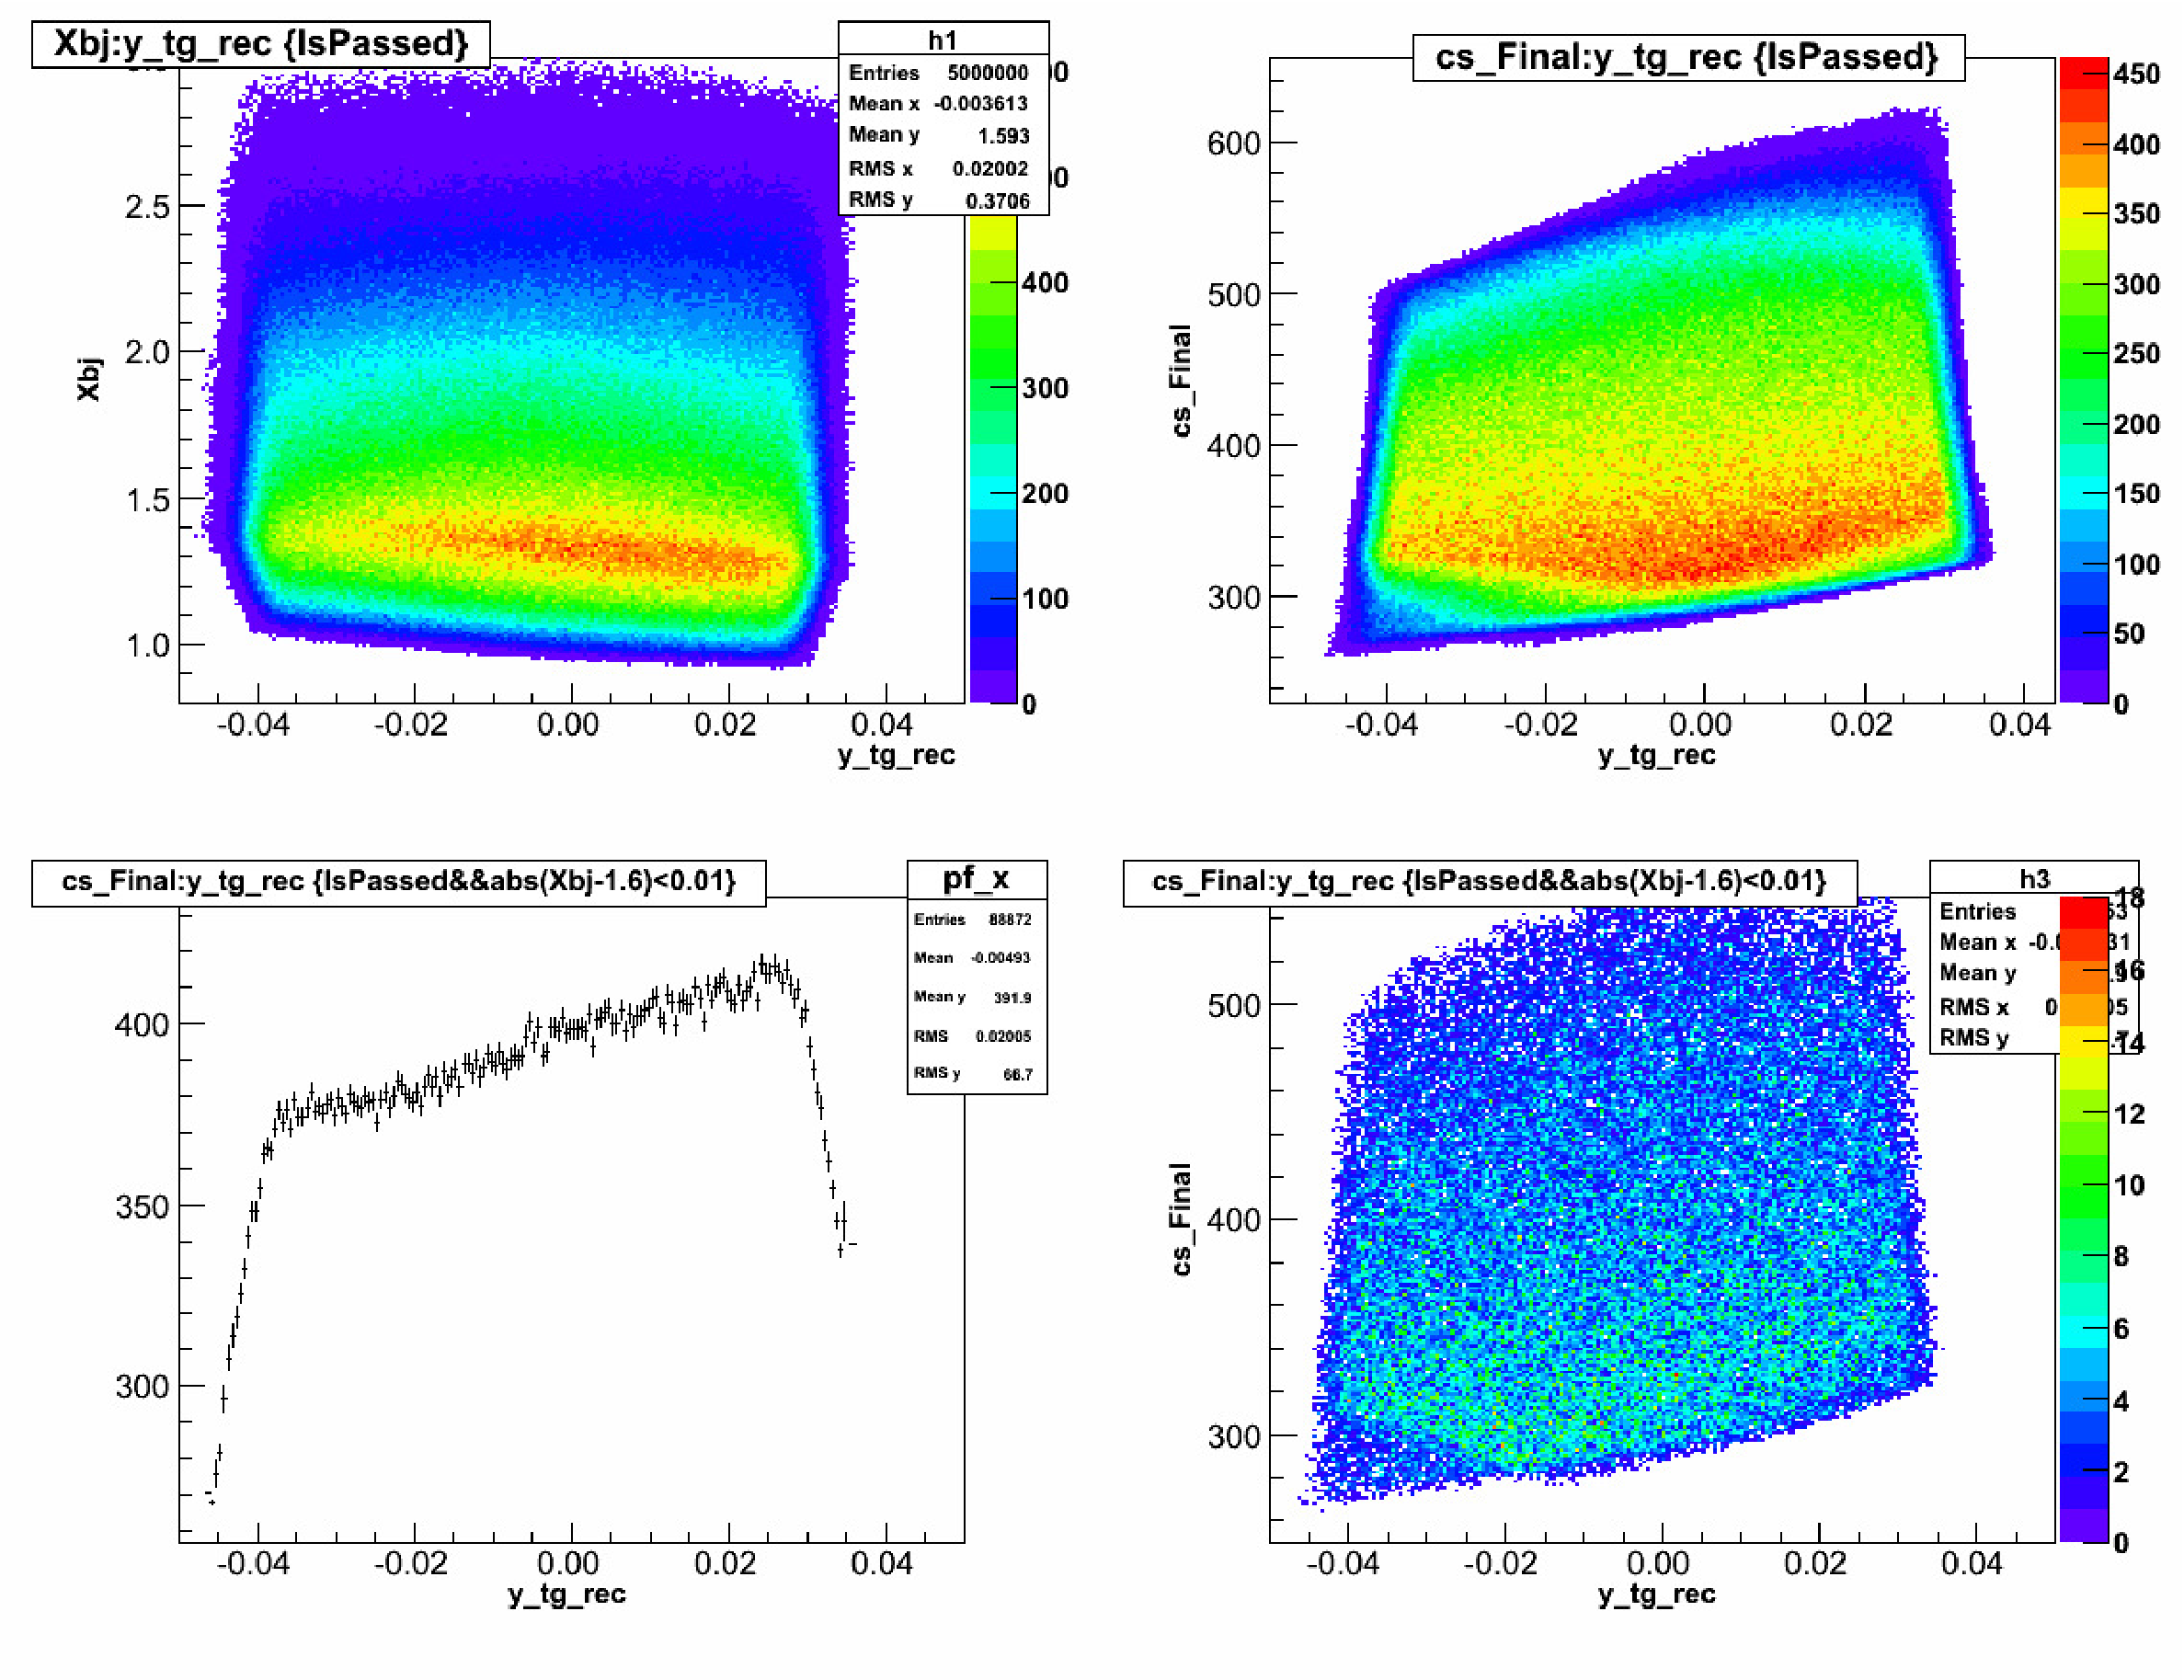
\includegraphics[type=pdf, ext=.pdf,read=.pdf,width=0.44\textwidth]{../figures/target/SAMC_Ytg_Xbj}
}

 \subfloat[w/ acceptance cuts]{
  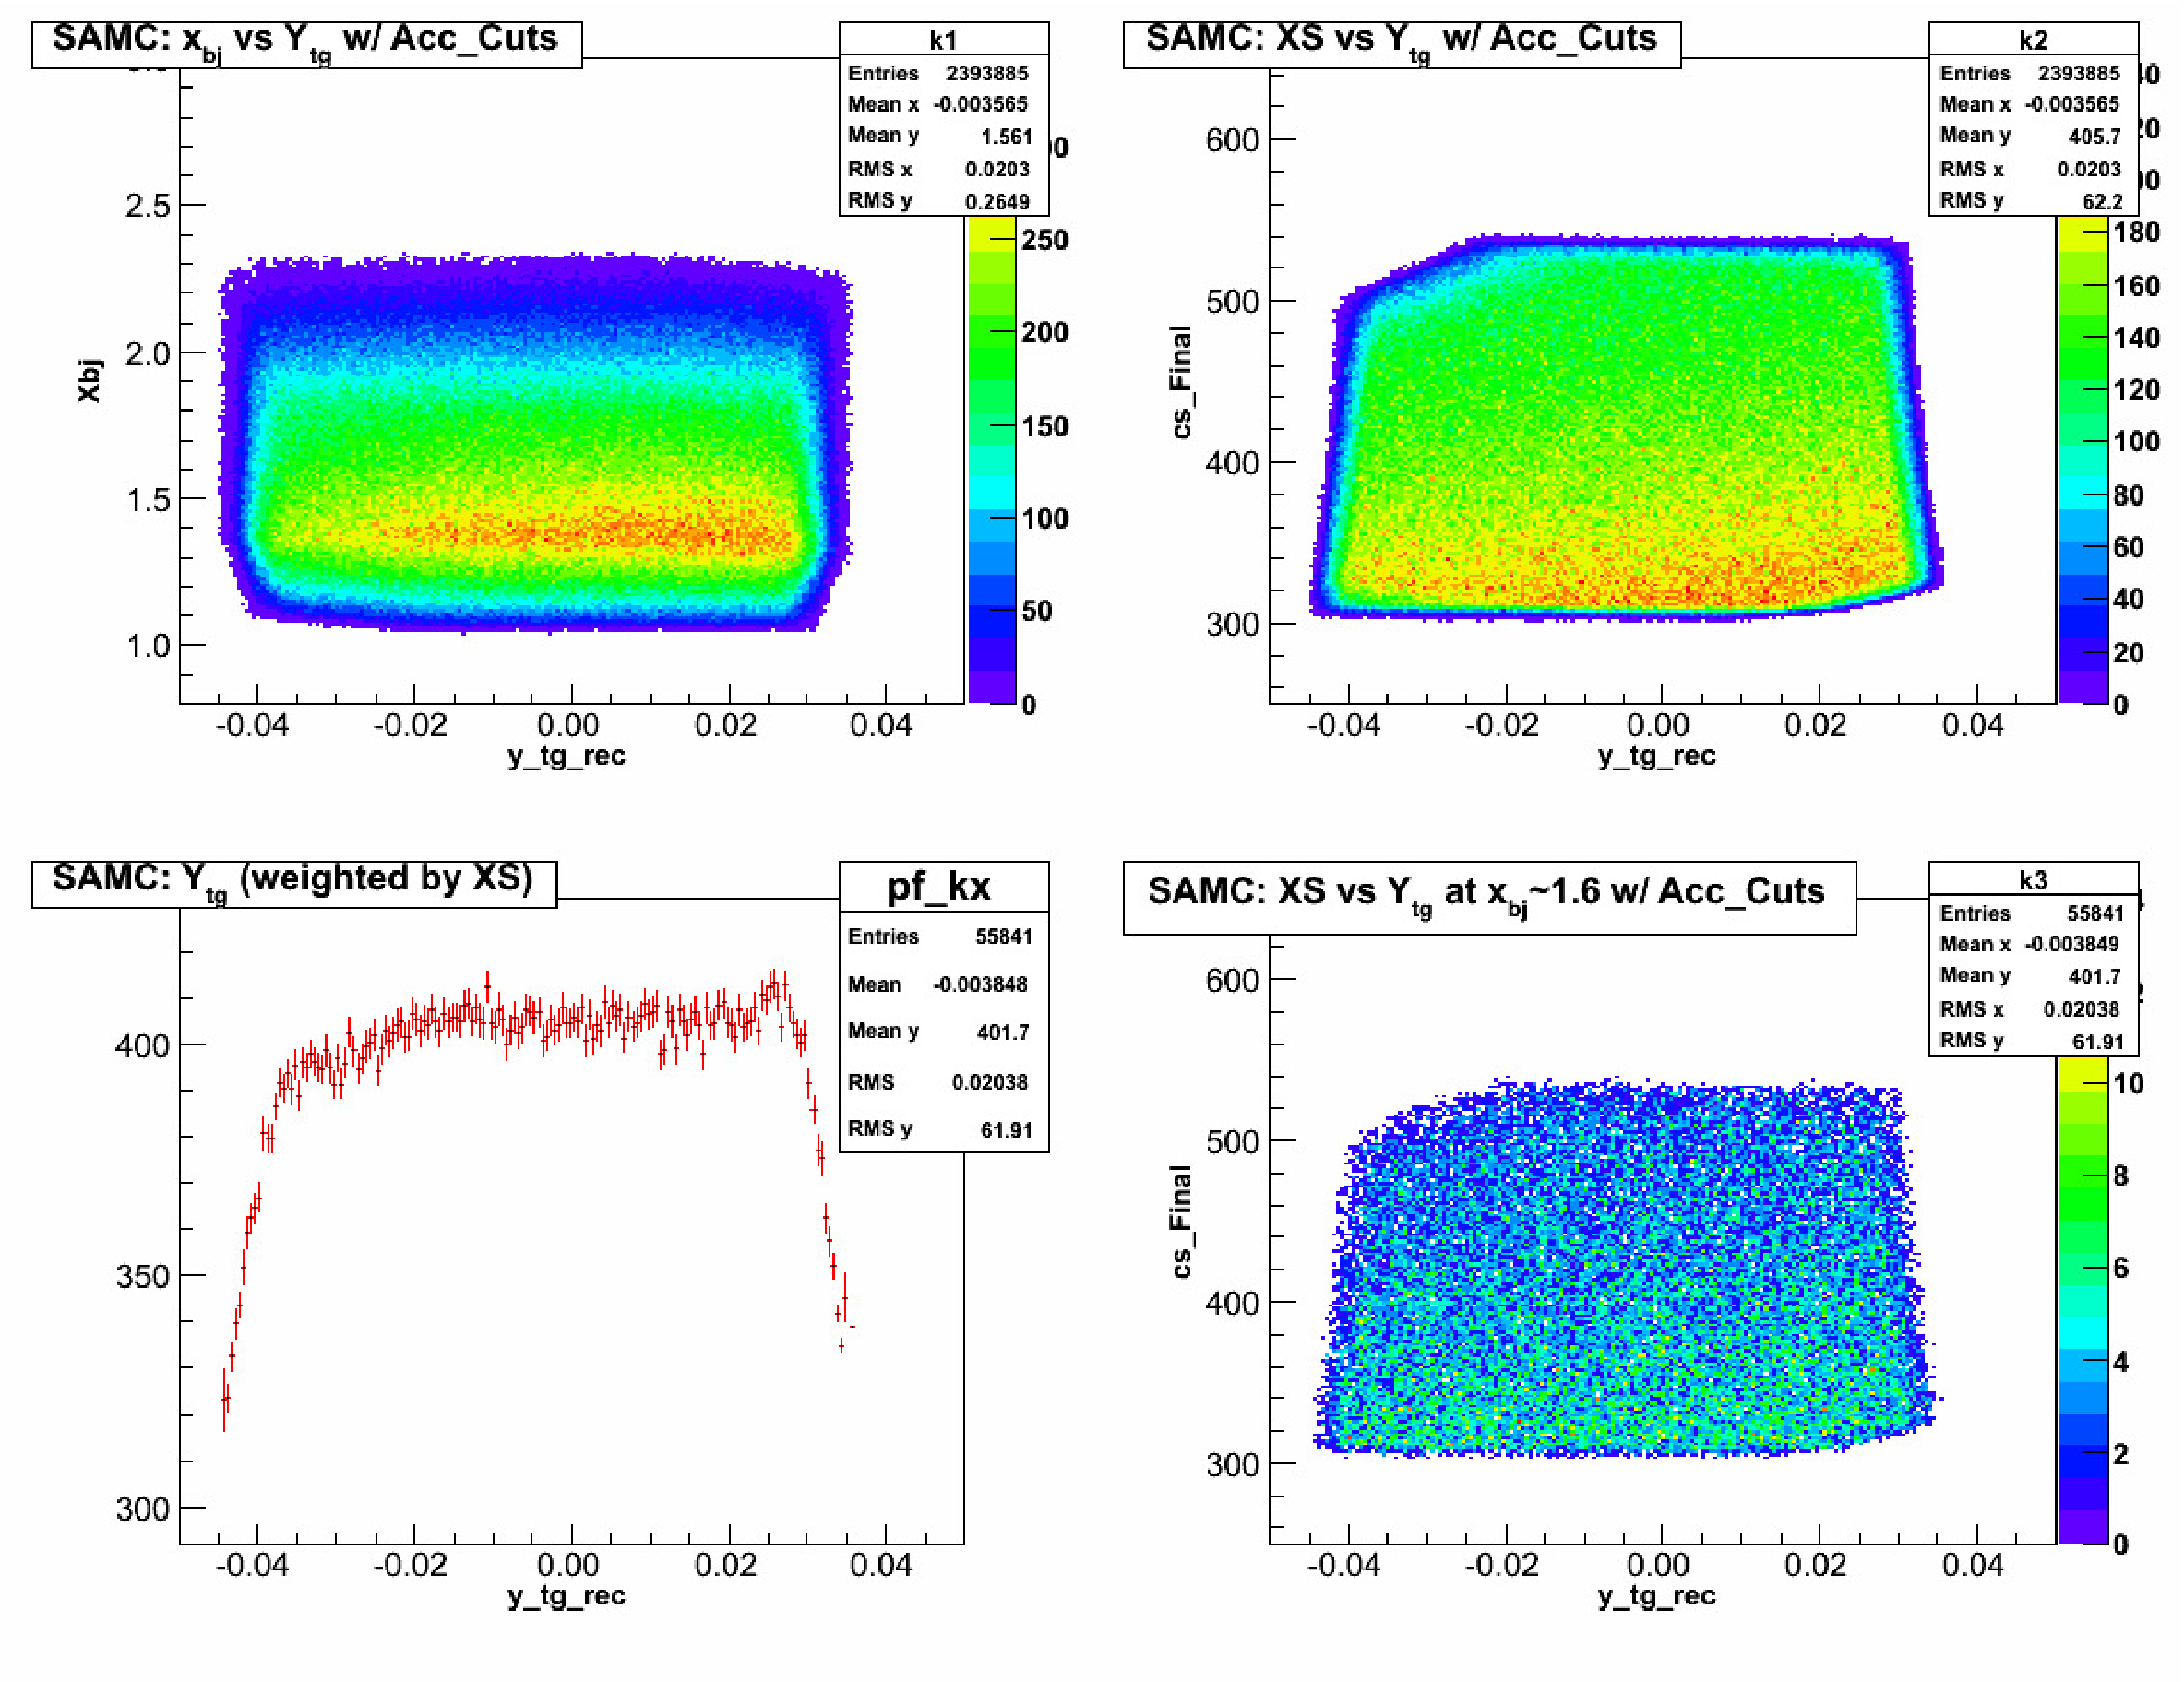
\includegraphics[width=0.45\textwidth]{../figures/target/SAMC_Ytg_Xbj_AccCuts}
}
  \caption[Cross section varying with along targets in simulation]{Cross section varying with along targets in one fine $x_{bj}$ bin using simulation data}
  \label{xs_bump_simu}
 \end{center}
\end{figure}

 Back to experiment data, we plot the correlation of $Y_{tg}$ and $x_{bj}$ (Fig.\ref{xs_bump_data}), where the profile of the 2-D histogram shows the dependence of $Y_{tg}$ on $x_{bj}$. From the plot at middle left, we also see that $x_{bj}$ does not affected by the bump. Base on those two examinations, we can conclude that when calculating raw cross sections, the target issue is not needed to be considered.

\begin{figure}[!ht]
 \begin{center}
  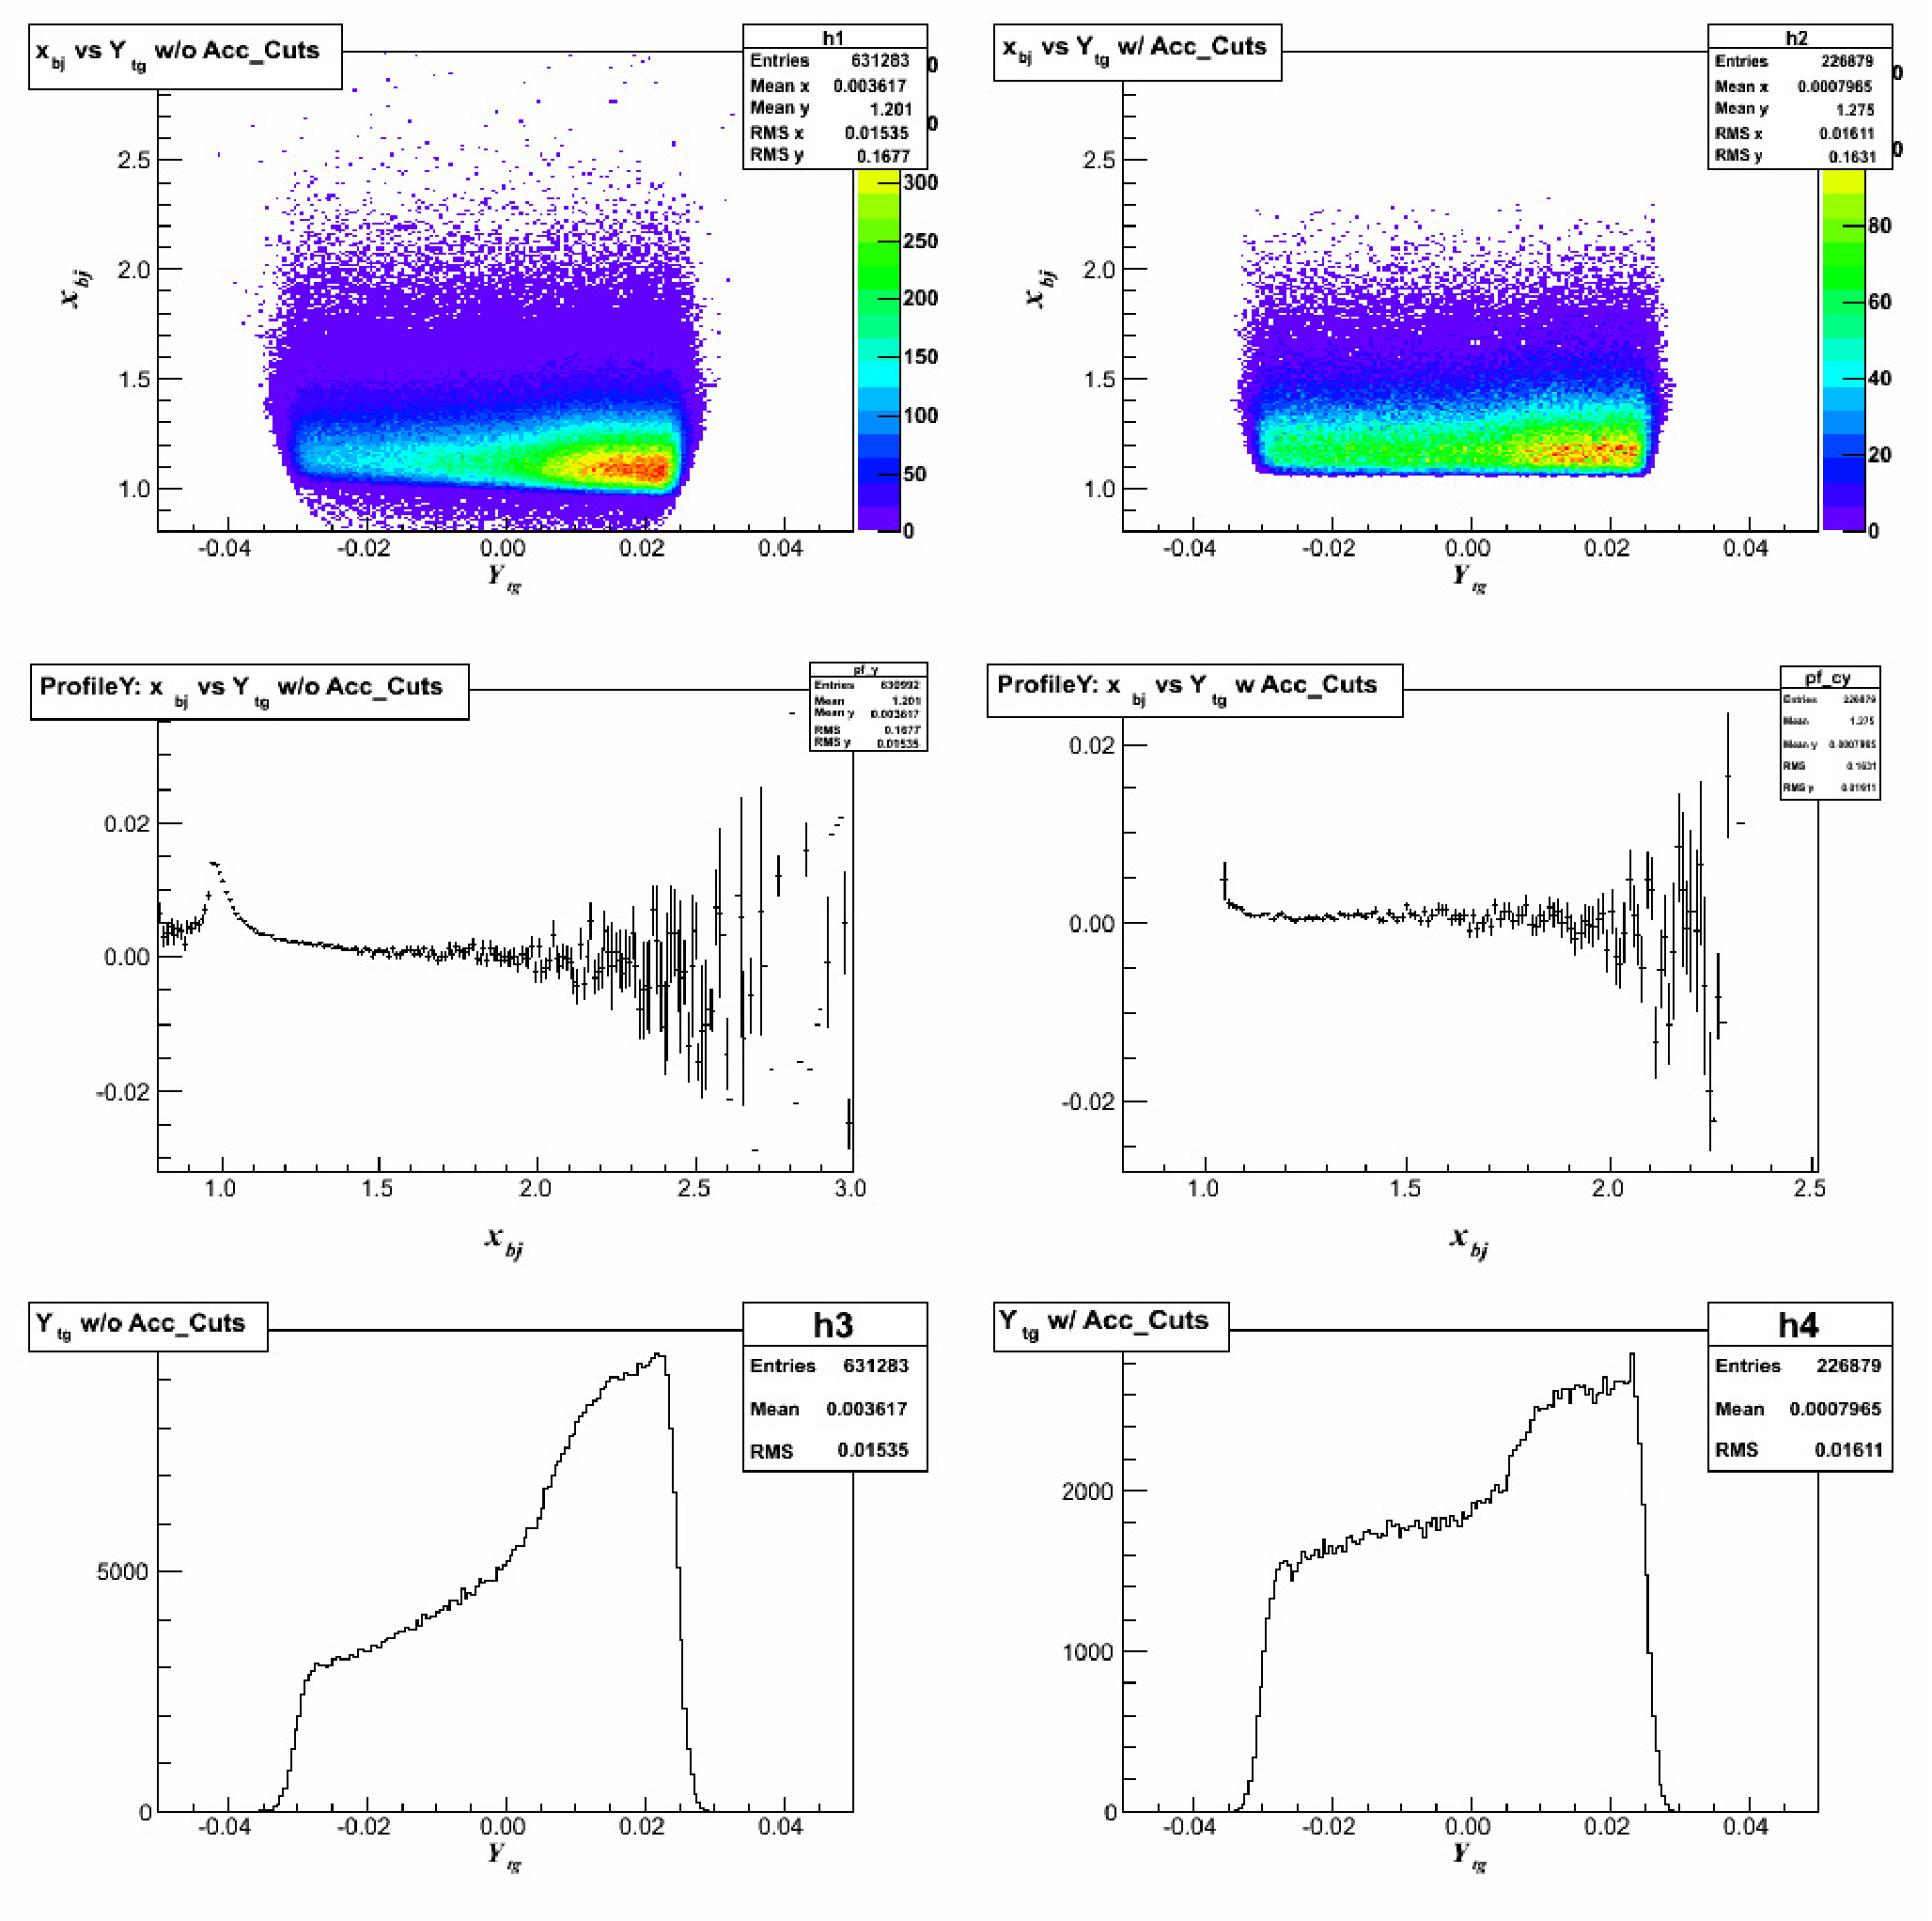
\includegraphics[type=pdf, ext=.pdf,read=.pdf,width=0.44\textwidth]{../figures/target/Data_He3_4085_Ytg_Xbj}
  \caption[Cross section varying with along targets in data]{Cross section varying with along targets in one fine $x_{bj}$ bin using experiment data}
  \label{xs_bump_data}
 \end{center}
\end{figure}

However, special treatments are required when we work on radiated cross sections. Transitionally we assume the reaction points always locates at the center of the target cell, which is a good estimation if the target density is uniform. It will be more complicate if parts of the target have high density and hence cause more reactions than other parts. The study heavily reply on a good radiated cross section model and a Monte Carlo tool. Detail description of how to treat the radiation correction using XEMC model can be found in Elog \#64 or the pdf file attached with this note. Basic idea is that we need to calculate cross sections for one setting ($E0, Ep$, and $\theta$), but in ten different locations in the target cell. In SAMC, we can modify the generator to generate more statistics on upstream part of long targets, to simulate the truth that more events coming out from the upstream part. Each event with specific $Y_{tg}$ value will look for its most close cross section value from the table. We can adjust the input until the distribution of $Y_{tg}$ for real data and simulation data completely agree with each other. When we calculate $N_{MC}^{i}$ in Eq\eqref{xs_eq}, the effect from long target bumps should be automatically corrected.

Once we obtain the radiated cross sections from experimental data, we need to know that how the average radiation correction should be with the good understanding of target density at different locations. Work base on this idea is still undergoing.


\end{document}

